\documentclass[12pt]{article}

\usepackage[margin=1in]{geometry}
\usepackage{amsmath,amssymb,amsthm}
\usepackage{booktabs}
\usepackage{titlesec}
\titleformat{\section}{\normalfont\bfseries}{\thesection.}{1em}{\MakeUppercase}
\titleformat{\subsection}{\normalfont\bfseries}{\thesubsection}{1em}{}
\usepackage{caption}
\captionsetup{labelsep=period,justification=raggedright,singlelinecheck=false}
\usepackage{natbib}
\usepackage[hidelinks]{hyperref}
\usepackage{setspace}

\bibpunct{(}{)}{;}{a}{}{,}

% Allow extra stretch in math-heavy paragraphs rather than overflowing the margin.
\emergencystretch=2em

% Let floats occupy more of a page before being pushed to a page of their own.
\renewcommand{\topfraction}{0.9}
\renewcommand{\bottomfraction}{0.8}
\renewcommand{\textfraction}{0.07}
\renewcommand{\floatpagefraction}{0.75}

\newtheorem{theorem}{Theorem}
\newtheorem{proposition}{Proposition}
\newtheorem{lemma}{Lemma}
\newtheorem{corollary}{Corollary}
\theoremstyle{definition}
\newtheorem{assumption}{Assumption}
\newtheorem{definition}{Definition}

\numberwithin{equation}{section}

% Captions sit above tables, and the article class leaves no space below a
% caption, so a caption running to two lines collides with \toprule.
\setlength{\abovecaptionskip}{10pt}
\setlength{\belowcaptionskip}{7pt}

\title{What Pre-Trends Cannot See:\\[2pt]
Testing for Treatment-Induced Recording Change\\[2pt]
with Few Clusters}

\author{Ethan Xie\thanks{Charter School of Wilmington, Wilmington, DE.
Email: \texttt{ethanxie@udel.edu}. Replication code, the simulation scripts and
the output files underlying the tables are at
\url{https://github.com/opxie1/what-pre-trends-cannot-see},
at the tagged release \texttt{v1.0}, which is immutable; the main
branch may move. The note to each table and figure names the
output file its entries are read from. The simulations are written in Python and need
version 3.11 or later with \texttt{numpy}, \texttt{scipy} and \texttt{pandas}.
They draw pseudorandom numbers from the NumPy PCG64 generator, seeded once per
replication by the CRC-32 checksum of a string naming the design cell and the
replication index, so that any cell can be regenerated on its own. Producing
every output file cited here takes $61.2$ minutes in total
(\texttt{results/inference/summary.json}, field
\texttt{runtime\_min\_total}).}}

\usepackage{pgfplots}
\pgfplotsset{compat=1.18}


\begin{document}

\begin{center}

{\large\bfseries Supplement to \emph{What Pre-Trends Cannot See:}}\\[2pt]

{\large\bfseries \emph{Testing for Treatment-Induced Recording Change with Few Clusters}}\\[8pt]

Ethan Xie

\end{center}

\vspace{6pt}

\noindent This supplement contains the proofs of every result in the paper, the simulation and application evidence behind the numbers the paper reports, the extended discussion of the related and applied literature, and the figure of exact size against the number of restrictions. Numbering follows the paper: a reference to Theorem 1 here is Theorem 1 there.

\vspace{10pt}

\setcounter{section}{0}

\renewcommand{\thesection}{S\arabic{section}}

\numberwithin{equation}{section}

\section{Proofs}

\begin{proof}[Proof of Lemma 1]
Write $s_1$ for the structure of the statement: latent outcomes $Y^{*}$
satisfying parallel trends, recording paths $m_c$ with $m_c(\ell)=0$ for
$\ell<0$, and unit by category terms $\mu_{ic}$, period by category terms
$\phi_{tc}$, recording noise $u_{itc}$ and cohort labels $G_i$. By Assumption
1 the observed panel under $s_1$ is
\begin{equation}
\label{eq:s1}
Y_{itc} = Y^{*}_{itc} + \mu_{ic} + \phi_{tc} + m_c(\ell_{it})D_{it} + u_{itc}.
\end{equation}

Construct $s_2$ on the same probability space by leaving
$\mu$, $\phi$, $u$ and $G$ unchanged, setting the recording paths to zero, and
replacing the latent untreated potential outcome by
\begin{equation}
\label{eq:dagger}
Y^{\dagger}_{itc}(\infty) = Y^{*}_{itc}(\infty) + m_c(t-g)\mathbf 1\{t \ge g\}
\qquad \text{on } \{G_i = g\},
\end{equation}
with treated potential outcomes shifted by the same increment, so that latent
treatment effects are unchanged. Since $s_2$ has no recording response, its
observed panel is $Y_{itc} = Y^{\dagger}_{itc} + \mu_{ic} + \phi_{tc} +
u_{itc}$, and substituting \eqref{eq:dagger} and $\ell_{it} = t - G_i$ returns
\eqref{eq:s1} cell by cell, pointwise on the underlying sample space. The two
structures therefore induce the same joint law of
$\{(Y_{itc})_{t,c}, G_i\}_{i \le N}$, not merely the same moments.

For the deviation induced by $s_2$, note that $s_1$ satisfies latent parallel
trends, so any departure under $s_2$ is the increment in \eqref{eq:dagger}.
Differencing it across $t$ and across cohorts in the definition of
$\Delta_c(g,t)$ gives $\Delta_c(g,t) = m_c(t-g)\mathbf 1\{t \ge g\}$, which is
(3.2). It vanishes for $t < g$ because $m_c(\ell) = 0$ for
$\ell < 0$, which is the no anticipation restriction in the recording layer.
\end{proof}

\begin{proof}[Proof of Corollary 1]
Let $\varphi$ be measurable with respect to $\sigma(\{(Y_{itc})_{t,c},G_i\}_{i
\le N})$. By Lemma 1 the law of that array is the same under $s_1$ and
$s_2$, so $E_{s_1}[\varphi] = E_{s_2}[\varphi]$. Under $s_2$ the deviation
$\Delta_c(g,t)$ is identically zero for $t<g$, so $s_2$ lies in the null of any
test whose null hypothesis restricts pre-treatment deviations. If $\varphi$ has
size $\alpha$ over that null then $E_{s_2}[\varphi] \le \alpha$, with equality
when the test is similar. Hence $E_{s_1}[\varphi] \le \alpha$, and equal to
$\alpha$ for a similar test, although $s_1$ carries a recording response of
arbitrary magnitude. The same argument applies to placebo in time statistics and
to leads and lags coefficient vectors, which are also functions of the observed
panel and the cohort labels.
\end{proof}

\begin{proof}[Proof of Proposition 1]
Adopt the normalization $\delta_{-1}=0$ and let the pre-period first differences
be $\delta_{s+1}-\delta_s$ for $s \le -2$, which are the differences a
relative magnitudes calibration reads. By Lemma 1 the deviation
equivalent to the recording response is $\delta_\ell = m_c(\ell)\mathbf 1\{\ell
\ge 0\}$, so $\delta_\ell = 0$ for every $\ell \le -1$ and every pre-period first
difference is exactly zero. Hence
$\max_{s \le -2}\lvert \delta_{s+1}-\delta_s \rvert = 0$, and the defining constraint
of (3.3) reads $\lvert \delta_{\ell+1}-\delta_\ell \rvert \le \bar M
\cdot 0 = 0$ for every $\ell \ge -1$ and every $\bar M \ge 0$. Together with
$\delta_{-1}=0$ this forces $\delta_\ell = 0$ for all $\ell$, so
$\Delta^{\mathrm{RM}}(\bar M) = \{0\}$ irrespective of $\bar M$.

The identified set for the target under a deviation class $\Delta$ is
$\{\,l'\beta_{\mathrm{post}} - l'\delta_{\mathrm{post}} : \delta \in \Delta\,\}$
with $\delta_{\mathrm{pre}}$ pinned at its population value. With
$\Delta^{\mathrm{RM}}(\bar M) = \{0\}$ this is the singleton
$\{\,l'\beta_{\mathrm{post}}\,\}$. By Lemma 1,
$\beta_c(\ell) = \vartheta_c(\ell) + m_c(\ell)$, so the singleton is
$\{\vartheta_c(\ell) + m_c(\ell)\}$ and excludes $\vartheta_c(\ell)$ whenever
$m_c(\ell) \ne 0$. Since the set is a point, no value of $\bar M$ returns an
interval containing the latent effect, and no breakdown value exists.
\end{proof}

\begin{proof}[Proof of Lemma 2]
Under Assumption 2 the regressor block in (4.1) is common
across categories after the two-way within transformation, so stacking the $C$
categories gives design matrix $[\,\mathbf{1}_C \otimes \tilde{X},\ \delta
\otimes \tilde{X}\,]$ with $\delta = (\delta_1,\dots,\delta_C)'$. Because
$\mathbf{1}_C'\delta = 0$ by the centering of $\delta$, the two blocks are
orthogonal, and the normal equations separate into
$(\mathbf{1}_C'\mathbf{1}_C) S \hat{\beta} = \sum_c \tilde{X}'\tilde{y}_c$ and
$(\delta'\delta) S \hat{\gamma} = \sum_c \delta_c \tilde{X}'\tilde{y}_c$.
Dividing by $C$ and $\sum_c \delta_c^2$ respectively and using $b_c =
S^{-1}\tilde{X}'\tilde{y}_c$ gives the stated expressions.
\end{proof}

\begin{proof}[Proof of Proposition 2]
By (5.1) the CR1 covariance of $\hat{\gamma}$ on the post block is
$\hat{V}_{PP} = \omega \sum_g \eta^f_{gP}\eta^{f\prime}_{gP}$ with $\omega =
\omega_2^{-1}G/(G-1)$. The within category residual is $e_{gc} = u_{gc} -
\tilde{X}_g S^{-1}\tilde{X}'u_c$ by Lemma 2, so $a^f_g = a_g -
S_gS^{-1}\sum_h a_h$ and $\eta^f_g = \eta_g - S^{-1}S_g\sum_h \eta_h$. Under
Assumption 3(ii), $S^{-1}S_g = I_q/G$, so $\eta^f_g = \eta_g -
\bar{\eta}$, the restriction to $P$ commutes with the correction, and
$\sum_g \eta^f_{gP}\eta^{f\prime}_{gP} = (G-1)\hat{S}_P$ while
$\hat{\gamma}_P - \gamma_P = G\bar{\eta}_P$. Substituting,
$$
W = \hat{\gamma}_P' \hat{V}_{PP}^{-1} \hat{\gamma}_P
  = \omega_2\, \bar{\eta}_P' \Big[\tfrac{1}{G-1}\textstyle\sum_g
    (\eta_{gP}-\bar{\eta}_P)(\eta_{gP}-\bar{\eta}_P)'\Big]^{-1}
    \bar{\eta}_P \, G
  = \omega_2 T^2 ,
$$
where the centering is the within category fitting correction and not a
consequence of imposing (4.2). This is an algebraic identity and does
not use Assumption 3(i).

For the distribution, Assumption 3(i) gives
\[
\sqrt{G}\,\bar{\eta}_P \sim N(0,\Sigma_{PP}),
\qquad
(G-1)\hat{S}_P \sim W_m(\Sigma_{PP}, G-1),
\]
independently, by Cochran's theorem applied to the i.i.d.\ Gaussian sample
$\eta_{1P},\dots,\eta_{GP}$. Hence $T^2$ is Hotelling's $T^2$ with dimension $m$
and $G-1$ degrees of freedom \citep{hotelling1931}, and the standard
transformation $\frac{G-m}{(G-1)m}T^2 \sim F(m,G-m)$ holds for $G-m\ge1$.
Substituting $T^2 = W/\omega_2$ gives (5.2).

For the last claim, write $\sum_g \eta^f_{gP}\eta^{f\prime}_{gP} = E'E$ with $E$
the $G \times m$ matrix whose $g$th row is $\eta^{f\prime}_{gP}$. Summing
$\eta^f_g = \eta_g - S^{-1}S_g\sum_h\eta_h$ over $g$ and using $\sum_g S_g = S$
gives $\sum_g \eta^f_g = 0$, so the columns of $E$ are orthogonal to
$\mathbf{1}_G$ and $\operatorname{rank}E \le \min(m, G-1)$. If $G - 1 < m$ the
meat is singular, $\hat{S}_P$ is not invertible, and the Hotelling
representation is unavailable.
\end{proof}

\begin{proof}[Proof of Corollary 2]
By (5.2) the exact size of the nominal chi-square test is
$\Pr\{F(m,G-m) > (G-m)c_m / (\omega_2(G-1)m)\}$ with $c_m =
\chi^2_{m,1-\alpha}$. Write $F(m,G-m) \overset{d}{=} (\chi^2_m/m) /
(\chi^2_{G-m}/(G-m))$ with the two chi squares independent, so the size equals
$\Pr\{\chi^2_m > c_m \,\omega_2^{-1}(G-1)^{-1}\chi^2_{G-m}\}$.

For (i), write $W \overset{d}{=} R\,\chi^2_m$ with $R = \omega_2 (G-1)/
\chi^2_{G-m}$ independent of $\chi^2_m$, so the size is $\mathbb{E}[h(R)]$ with
$h(x) = \Pr\{\chi^2_m > c_m/x\}$ and $h(1) = \alpha$. Put $\nu = G-1$ and
$d = G-m$. At fixed $m$, $\mathbb{E}[R-1] = (m+1)/\nu - (1-\omega_2) +
O(\nu^{-2})$ and $\mathbb{E}[(R-1)^2] = 2/\nu + O(\nu^{-2})$, using
$\mathbb{E}[\chi_d^{-2k}] = \prod_{j=1}^{k}(d-2j)^{-1}$ for $d > 2k$ and
$G(1-\omega_2) = O(1)$. The same formula gives the third central moment of
$1/\chi^2_d$ as $16/\{(d-2)^3(d-4)(d-6)\}$ for $d > 6$, whence the signed third
moment $\mathbb{E}[(R-1)^3] = O(\nu^{-2})$.

A second order expansion does not deliver the remainder. Bounding it by
$\sup|h'''|\,\mathbb{E}|R-1|^3$ gives $O(\nu^{-3/2})$, because the absolute
third moment, unlike the signed one, gains nothing from cancellation. Expand
instead to third order with a fourth order Lagrange remainder. Outside
$|R-1| \le 1/2$ the contribution to $\mathbb{E}[h(R)]$ is exponentially small in
$\nu$, since $h$ is bounded by one and the chi square Chernoff bound gives
$\Pr(|R-1| > 1/2) \le e^{-c\nu}$ for some $c>0$. Inside,
$\sup_{|x-1| \le 1/2}|h''''(x)|$ is finite and $\mathbb{E}[(R-1)^4] =
3\{\mathbb{E}[(R-1)^2]\}^2 + O(\nu^{-3}) = 12/\nu^2 + O(\nu^{-3})$, so the
third order term and the remainder are both $O(\nu^{-2})$.

Substituting the moments with $h'(1) = c_m f_m(c_m)$ and $h''(1) =
-c_m^2 f_m'(c_m) - 2 c_m f_m(c_m)$, and using $f_m'(x) = f_m(x)
\{(m/2-1)/x - 1/2\}$ so that $c_m^2 f_m'(c_m) = c_m f_m(c_m)
\{(m/2-1) - c_m/2\}$, the bracket collapses to
$$
h'(1)\,\mathbb{E}[R-1] + \tfrac{1}{2}h''(1)\,\mathbb{E}[(R-1)^2]
= c_m f_m(c_m)\Big[\frac{m+c_m}{2\nu} - (1-\omega_2)\Big],
$$
which is the stated expansion. At the design of Section 9 with
$G = 51$ and $C = 3$, where $\omega_2 = 0.9981$, the two terms in that bracket
are $0.354$ and $1.9 \times 10^{-3}$ at $m = 13$ and $\alpha = 0.05$, and
$G(1-\omega_2)$ is at most $0.098$ over the twelve designs of Table
2
(\texttt{results/inference/anatomy\_table.csv}).

For (ii), take logarithms. The event is $\log \chi^2_m - \log \chi^2_{G-m} >
\log c_m - \log(\omega_2(G-1))$. With $m \to \infty$, $\log\chi^2_m$ is
asymptotically normal with mean $\log m - 1/m + O(m^{-2})$ and variance $2/m$,
and similarly for $\log\chi^2_{G-m}$ with $G - m \to \infty$. Standardizing and
using $\log c_m = \log m + \sqrt{2/m}\,z_{1-\alpha} + o(m^{-1/2})$ gives size
$\to \Phi(\chi - z_{1-\alpha})$ with $\chi = \lim \sqrt{m/2}\,\log\{(G-1)/(G-m)\}$.
Expanding $\log\{(G-1)/(G-m)\} = (m-1)/(G-1) + O((m/G)^2)$ gives $\chi_{m,G} =
m^{3/2}/(\sqrt{2}G) + o(1)$ when $m^{5/2}/G^2 \to 0$. If $m/G \to r \in (0,1)$
then $\log\{(G-1)/(G-m)\} \to -\log(1-r) > 0$ and $\chi_{m,G} \to \infty$, so
the size tends to one.
\end{proof}

\begin{proof}[Proof of Lemma 3]
Under Assumption 2 the two-way within transformation is the same
operator for every category, so relabelling the arrays gives
$\hat{\Sigma}(\mathcal{D}_\sigma)_{ck} = \hat{\Sigma}_{\sigma(c)\sigma(k)}$ and
hence $L(\mathcal{D}_\sigma)_{ck} = L_{\sigma(c)\sigma(k)}$. Substituting
$j = \sigma(k)$ maps $\{k \ne c\}$ bijectively onto $\{j \ne \sigma(c)\}$, and
substituting $(j,l) = (\sigma(k),\sigma(l))$ maps $\{k \ne l,\; k,l \ne c\}$
bijectively onto $\{j \ne l,\; j,l \ne \sigma(c)\}$, so both averages in
(6.1) are evaluated at the relabeled index and
$\hat{a}_c(\mathcal{D}_\sigma) = \hat{a}_{\sigma(c)}(\mathcal{D})$. The
geometric mean scaling divides by $\exp\{C^{-1}\sum_j \hat{a}_j\}$, which is
$\sigma$-invariant, so $\hat{\rho}_c(\mathcal{D}_\sigma) =
\hat{\rho}_{\sigma(c)}(\mathcal{D})$. The retained set and the normalized arrays
are therefore relabeled with the loadings.
\end{proof}

\begin{proof}[Proof of Theorem 1]
The argument is the classical group invariance construction; see
\citet[Ch.~15]{lehmann2005testing}. Order invariance of $\mathcal{T}$ gives, for
every $\pi \in S_C$, $\mathcal{T}(\mathcal{D},\delta_\pi) =
\mathcal{T}(\mathcal{D}_{\pi^{-1}},\delta)$ where $\mathcal{D}_{\pi^{-1}} =
(\mathcal{Y}_{\pi^{-1}(1)},\dots,\mathcal{Y}_{\pi^{-1}(C)})$: the statistic is
computed from the multiset $\{(\delta_{\pi(c)},\mathcal{Y}_c)\}_c$, and
reindexing by $j = \pi(c)$ turns this into
$\{(\delta_j,\mathcal{Y}_{\pi^{-1}(j)})\}_j$.

Under Assumption 4, $\mathcal{D}_{\pi^{-1}} \overset{d}{=}
\mathcal{D}$ conditional on $\mathcal{Z}$ for each fixed $\pi$. The invariance
the argument needs is under right translation of the index. Writing
$f(\cdot) = \mathcal{T}(\cdot,\delta)$, so that $T(\pi) =
f(\mathcal{D}_{\pi^{-1}})$, the substitution $\pi \mapsto \pi\sigma$ gives
$$
T(\pi\sigma) = f\big(\mathcal{D}_{(\pi\sigma)^{-1}}\big)
              = f\big(\mathcal{D}_{\sigma^{-1}\pi^{-1}}\big)
              = f\big((\mathcal{D}_{\sigma^{-1}})_{\pi^{-1}}\big),
$$
so $(T(\pi\sigma))_{\pi}$ is the same fixed measurable function of
$\mathcal{D}_{\sigma^{-1}}$ that $(T(\pi))_{\pi}$ is of $\mathcal{D}$. By
Assumption 4, $\mathcal{D}_{\sigma^{-1}} \overset{d}{=}
\mathcal{D}$ conditional on $\mathcal{Z}$, whence
$(T(\pi\sigma))_{\pi} \overset{d}{=} (T(\pi))_{\pi}$ for every
$\sigma \in S_C$. Left translation does not have this property, since
$T(\sigma\pi) = f(\mathcal{D}_{\pi^{-1}\sigma^{-1}})$ is not a fixed function
of any one relabelling of $\mathcal{D}$, and it is right translation that the
counting below uses.

We bound $\Pr(\hat{p} \le \alpha)$ for the $\hat{p}$ of Definition
2 directly, which covers ties. For $\sigma \in S_C$ put
$N(\sigma) = \#\{\pi' \in S_C : T(\pi') \ge T(\sigma)\}$ and $\mathcal{A} =
\{\sigma : N(\sigma) \le \alpha M\}$, so the test rejects exactly on the event
$\mathrm{id} \in \mathcal{A}$. If $\mathcal{A}$ is not empty, let $\sigma^*$
attain the smallest value of $T$ on it. Every $\sigma \in \mathcal{A}$ has
$T(\sigma) \ge T(\sigma^*)$, so $\mathcal{A} \subseteq \{\pi' : T(\pi') \ge
T(\sigma^*)\}$ and $|\mathcal{A}| \le N(\sigma^*) \le \alpha M$, hence
$|\mathcal{A}| \le \lfloor \alpha M \rfloor$ because $|\mathcal{A}|$ is an
integer. Write $\phi(t) = \mathbf{1}\{\#\{\pi : t_\pi \ge t_{\mathrm{id}}\}
\le \alpha M\}$ for a vector $t$ indexed by $S_C$, so that the rejection
indicator is $\phi\big((T(\pi))_\pi\big)$. Because $\pi \mapsto \pi\sigma$ is
a bijection of $S_C$, the vector $(T(\pi\sigma))_\pi$ carries $T(\sigma)$ in
its identity coordinate and the same multiset of values, so
$\phi\big((T(\pi\sigma))_\pi\big) = \mathbf{1}\{N(\sigma) \le
\alpha M\}$, and summing over $\sigma$ gives $\sum_{\sigma \in S_C}
\phi\big((T(\pi\sigma))_\pi\big) = |\mathcal{A}|$. Taking expectations
conditional on $\mathcal{Z}$ and applying exchangeability to each term,
$$
M \Pr(\hat{p} \le \alpha \mid \mathcal{Z})
= \mathbb{E}\big[\,|\mathcal{A}| \,\big|\, \mathcal{Z}\big]
\le \lfloor \alpha M \rfloor ,
$$
so $\Pr(\hat{p} \le \alpha \mid \mathcal{Z}) \le \lfloor \alpha M\rfloor/M
\le \alpha$. Averaging over $\mathcal{Z}$ preserves the bound.

Two cases sharpen it. When the $M$ values are almost surely distinct, $N$ takes
each of $1,\dots,M$ exactly once, so $|\mathcal{A}| = \lfloor \alpha M \rfloor$
and the bound holds with equality. When they fall into $M/\mathfrak{m}$ groups of
exactly $\mathfrak{m}$ equal values, distinct across groups, which is what
Proposition 3(ii) gives with $\mathfrak{m} = 2$ for the
two sided Wald statistic, $N$ takes each of $\mathfrak{m}, 2\mathfrak{m},\dots,M$ with
multiplicity $\mathfrak{m}$, so $|\mathcal{A}| = \mathfrak{m}\lfloor \alpha
M/\mathfrak{m} \rfloor$ and $\Pr(\hat{p} \le \alpha) = \mathfrak{m}\lfloor \alpha
M/\mathfrak{m}\rfloor/M$. In either case the randomized version rejects with
probability one on
$\{\hat{p} \le \alpha_-\}$, whose probability is $\alpha_-$, and with
probability $(\alpha-\alpha_-)/(\alpha_+-\alpha_-)$ on $\{\hat{p} = \alpha_+\}$,
whose probability is $\alpha_+-\alpha_-$, so its size is $\alpha$.

For the Monte Carlo reference set of Definition 2, replace $S_C$ by
$\mathcal{R} = \{\mathrm{id},\pi_2,\dots,\pi_B\}$. Because $\pi_2,\dots,\pi_B$
are i.i.d.\ uniform on $S_C$ and drawn independently of the data, the vector
$(T(\pi))_{\pi \in \mathcal{R}}$ is exchangeable conditional on $\mathcal{Z}$
under Assumption 4, and the rank argument above gives
$\Pr(\text{reject}) \le \alpha$ with equality at
$\mathfrak{m}\lfloor \alpha B/\mathfrak{m}\rfloor/B$.
\end{proof}

\begin{proof}[Proof of Proposition 3]
(i) Every $\pi \in \mathrm{Stab}(\delta)$ satisfies $\delta_\pi = \delta$ and
hence $T(\pi) = T(\mathrm{id})$, so the numerator of $\hat{p}$ is at least
$|\mathrm{Stab}(\delta)|$ on the exhaustive reference set, and
$\mathrm{Stab}(\delta)$ is the direct product of the symmetric groups on the
tied groups of $d$, of order the product of their factorials. On the Monte Carlo
reference set the identity alone gives $\hat{p} \ge 1/B$.

(ii) Because the multiset $\{\delta_c\}$ is symmetric about zero, pick an
involution $r \in S_C$ matching each $c$ with $\delta_c = v > 0$ to some $c'$
with $\delta_{c'} = -v$ and fixing every $c$ with $\delta_c = 0$; then
$\delta_{r(c)} = -\delta_c$ for all $c$, and $r \ne \mathrm{id}$ because
$\delta$ is not identically zero. With equally spaced $d$ we may write
$\delta_c = s\,(c - \frac{C+1}{2})$ for a scale $s>0$ and take $r(c) = C+1-c$.
Precomposition negates the label vector:
$(\delta_{r \circ \pi})_c = \delta_{r(\pi(c))} = -\delta_{\pi(c)}$, so
$\delta_{r\circ\pi} = -\delta_\pi$. Evenness of $\mathcal{T}$ then gives
$T(r\circ\pi) = T(\pi)$ for every $\pi$. The map $\pi \mapsto r\circ\pi$ is left
translation by an involution other than the identity, hence a fixed point free
involution on $S_C$, so the $M$ values fall into $M/2$ equal pairs, and
$r\circ\mathrm{Stab}(\delta)$ is disjoint from $\mathrm{Stab}(\delta)$ because
$r \notin \mathrm{Stab}(\delta)$. The numerator of $\hat{p}$ is therefore at
least $2|\mathrm{Stab}(\delta)|$.

For the Wald statistic, $\hat{\gamma}(-\delta) = -\hat{\gamma}(\delta)$ by
Lemma 2, each cluster score is odd in $\delta$, and the CR1
covariance is quadratic in the cluster scores, so $\hat{V}_\gamma(-\delta) =
\hat{V}_\gamma(\delta)$ and the quadratic form is unchanged.

(iii) Rejection at level $\alpha$ requires some attainable $\hat p \le \alpha$,
hence $2|\mathrm{Stab}(\delta)|/C! \le \alpha$ in the even case and
$|\mathrm{Stab}(\delta)|/C! \le \alpha$ otherwise, which reduce to $2/C! \le
\alpha$ and $1/C! \le \alpha$ when $d$ has no ties.
\end{proof}

\begin{proof}[Proof of Theorem 2]
For the first claim, replace $S_C$ in the proof of Theorem 1 by
the finite group $\mathcal{E} = \{-1,+1\}^G$ acting by coordinatewise sign
change. That proof uses only finiteness of the group and invariance of the data
law under right translation by each of its elements, both of which the sign
symmetry hypothesis supplies. $\mathcal{E}$ is abelian, so the distinction
between left and right translation that the proof of Theorem 1
turns on is vacuous here.

For the second claim, let $u_{gc}$ denote the cluster-$g$ category-$c$ errors
under (4.2), taken before the two-way within transformation, and build
the infeasible contribution from them,
$$
\zeta^0_g = \frac{\big(S^{-1}\sum_c \delta_c \tilde{X}_g' u_{gc}\big)_P}
{\sum_c \delta_c^2} .
$$
Using the raw rather than the within transformed errors matters here and costs
nothing. It matters because the two-way within projection subtracts period
means, which pool across clusters, so contributions formed from the
within transformed errors are dependent across $g$. It costs
nothing because $\tilde{X}'\Pi = \tilde{X}'$, so the aggregate is unchanged and
$\sum_g \zeta^0_g = \hat{\gamma}_P - \gamma_P$ still holds. Each $\zeta^0_g$ is
then a fixed linear functional of cluster $g$'s errors alone, so independence
across $g$ together with symmetry of each summand about zero gives
$(\epsilon_g \zeta^0_g)_g \overset{d}{=} (\zeta^0_g)_g$ for every
$\epsilon \in \mathcal{E}$.

For the third claim, write $z^r_g$ for the cluster-$g$ score of the $\gamma$
block from the fit with (4.2) imposed, so the feasible contribution is
$\zeta_g = (S^{-1}z^r_g)_P/\sum_c \delta_c^2$. It replaces the errors by the
restricted residuals, which subtracts a term $S^{-1}S_g[\sum_h(\cdot)_h]$. The
factor $\|S_g\|/\|S\|$ is $O(G^{-1})$ and it multiplies a sum of $G$ cluster
contributions, which is $O_p(G^{1/2})$ times a single one; relative to $\zeta_g$
itself the discrepancy is therefore $O_p(G^{-1/2})$.

Asymptotic level $\alpha$ does not follow from an approximate symmetry argument
over $\mathcal{E}$. The results of \citet{canay2017randomization} hold for a
randomization group whose cardinality is fixed in the sample size, and
$|\mathcal{E}| = 2^G$ grows with $G$. We argue it instead as a statement about
the conditional law of the randomization distribution. Assume (W1) the cluster
blocks $(\tilde{X}_g, \{u_{gc}\}_c)$ are independent across $g$ with
$\mathbb{E}[z^0_g] = 0$ under (4.2) and uniformly bounded moments of
order strictly greater than four, where $z^0_g = \sum_c \delta_c
\tilde{X}_g'u_{gc}$; (W2) $\max_g \|S_g\|/\|S\| \to 0$ and $G^{-1}S \to
\bar{S} \succ 0$; and (W3) $G^{-1}\sum_g \mathbb{E}[z^0_g z^{0\prime}_g] \to
\Sigma_z \succ 0$ on the block $P$. The sign-change distribution is the
null imposed Rademacher wild cluster bootstrap of \citet{cameron2008bootstrap}
in score form. Conditional on the data, $G^{-1/2}\sum_g \epsilon_g z^r_g$ is a
sum of $G$ independent mean zero terms with conditional variance $G^{-1}\sum_g
z^r_g z_g^{r\prime}$, which converges in probability to $\Sigma_z$ under (W1) to
(W3), and (W1) with (W2) gives the conditional Lyapunov condition. The
conditional bootstrap central limit theorem of \citet{djogbenou2019asymptotic}
then gives the randomization distribution of the statistic the same $\chi^2_m$
limit, conditionally in probability, that the statistic itself has under
(4.2). The randomization $p$ value is therefore asymptotically
uniform.
\end{proof}

\begin{proof}[Proof of Corollary 3]
Under the alternative $\gamma = \kappa k$, Lemma 2 gives
$\hat{\gamma} = \sum_c \delta_c b_c/\Sigma_\delta^2$ with $\mathbb{E}[b_c] =
(\beta_\ell)_{\ell \in L} + \delta_c \kappa k$, and with homoskedastic
categories independent across
$c$, $\operatorname{Var}(b_c) = \sigma^2 S^{-1}$. Since $\sum_c \delta_c = 0$,
$\hat{\gamma}$ has mean $\kappa k$ and covariance $(\sigma^2/\Sigma_\delta^2)
S^{-1}$, so on the post-treatment block $V = \operatorname{Var}(\hat{\gamma}_P)
= (\sigma^2/\Sigma_\delta^2)[S^{-1}]_{PP}$ and, by the definition of $I_k$ in
Section 8, $\kappa^2 k_P'V^{-1}k_P = \kappa^2 \Sigma_\delta^2
I_k/\sigma^2$.

The first expression in (8.2) is the minimum detectable response of the
infeasible Wald statistic that uses $V$ in place of an estimate. That statistic
is noncentral chi-square with $m$ degrees of freedom and noncentrality
$\lambda = \kappa^2 \Sigma_\delta^2 I_k/\sigma^2$; setting $\lambda =
\lambda^*(\alpha,\beta,m)$ and solving for $\kappa$ gives it. The feasible CR1
Wald statistic does not have that law. The identity in the proof of Proposition
2 uses no distributional assumption and holds under the
alternative with $\bar{\eta}_P$ replaced by $\hat{\gamma}_P/G$, so under
Assumptions 2 and 3 the feasible statistic is $\omega_2$ times
a noncentral Hotelling $T^2$ with dimension $m$ and $G-1$ degrees of freedom.
Equation (8.2) therefore understates the minimum detectable response of
the feasible test twice, through the critical value, as Section 8
records, and through the distribution under the alternative.

For the directed statistic, $t$ is standard normal under (4.2) and
normal with unit variance and mean $\kappa \sqrt{\Sigma_\delta^2 I_k}/\sigma$
under the alternative, so power $1-\beta$ at level $\alpha$ requires that mean
to equal $z_{1-\alpha}+z_\beta$, which gives the second expression.
\end{proof}

\begin{proof}[Proof of Theorem 3]
Two configurations $(b_c)_c$ with the same contrast vector $(b_c - \bar{b})_c$
differ by a shift common to all categories, so the $C-1$ contrasts are a maximal
invariant and an invariant test is a function of them. The maximal invariant is
the full contrast vector, of dimension $(C-1)q$, and not $\hat{\gamma}_P$.
Decompose the contrast space orthogonally in the category index into the
direction $\delta$ and its complement. The $\delta$-component is
$\hat{\gamma} = \sum_c \delta_c b_c/\sum_c \delta_c^2$, with mean $\kappa k$.
The remaining $C-2$ contrasts have mean zero for every $\kappa$, so they are
ancillary for $\kappa$, and because $\Sigma$ does not vary with $c$ they are
uncorrelated with $\hat{\gamma}$ and, being jointly Gaussian with it,
independent of it. Write $A$ for that block.

Conditional on $A = a$, the law of $\hat{\gamma}_P$ is $N(\kappa k_P, V)$ and
does not depend on $a$. Its density in $\kappa$ is proportional to
$\exp\{\kappa k_P'V^{-1}\hat{\gamma}_P - \tfrac{1}{2}\kappa^2 k_P'V^{-1}k_P\}$
relative to the $\kappa = 0$ density, a one parameter exponential family with
natural parameter $\kappa$ and natural sufficient statistic $U =
k_P'V^{-1}\hat{\gamma}_P$, which has monotone likelihood ratio in $\kappa$. By
the Karlin--Rubin theorem \citep{lehmann2005testing} the conditional test
rejecting for large $U$ is uniformly most powerful at every conditional level,
and at conditional level $u$ its power is $\Psi(u) = \Phi(\mu + \Phi^{-1}(u))$
with $\mu = \kappa\sqrt{k_P'V^{-1}k_P} > 0$.

An invariant test may still randomize its level over the ancillary block, taking
conditional level $\alpha(A)$ with $\mathbb{E}[\alpha(A)] = \alpha$, and ruling
that out is the remaining step. Differentiating, $\Psi'(u) =
\exp\{-\mu^2/2 - \mu\Phi^{-1}(u)\}$, which is strictly decreasing in $u$, so
$\Psi$ is strictly concave on $(0,1)$ and Jensen's inequality gives
$\mathbb{E}[\Psi(\alpha(A))] \le \Psi(\alpha)$, with equality if and only if
$\alpha(\cdot)$ is almost surely constant. The unconditional power of an
invariant level-$\alpha$ test is therefore at most $\Psi(\alpha)$, attained by
$\alpha(\cdot) \equiv \alpha$. Standardizing $U$ by $\sqrt{k_P'V^{-1}k_P}$ gives
$t \sim N(\kappa\sqrt{k_P'V^{-1}k_P},1)$, from which the critical value and the
stated power function follow.
\end{proof}

\section{Additional simulation evidence}

\paragraph{The exact null law in the ideal experiment.} Assumption 3 is
not satisfied by the panel design, so Proposition 2 is checked
separately in an experiment built to satisfy it: cluster contributions drawn
i.i.d.\ $N(0,\Sigma)$ with $m = 13$, $\Sigma$ redrawn for each of three seeds,
and $60{,}000$ replications in total at each $G$. The identity
$W = \omega_2 T^2$ holds to a maximum relative error of $4.0 \times 10^{-14}$
at $G = 20$ and $1.3 \times 10^{-15}$ at $G = 100$. Referring the statistic to
the $F$ law of (5.2) at the nominal $G$ gives null rejection rates
of $0.0495$, $0.0489$, $0.0502$ and $0.0499$ at $G = 20$, $30$, $51$ and
$100$, quoted to four decimals here because the claim is that they are
indistinguishable from the nominal $0.05$ rather than merely close to it. Kolmogorov--Smirnov tests of the resulting $p$ values against the uniform
return $p = 0.81$, $0.02$, $0.06$ and $0.77$ at those four $G$, so the pooled
$G = 30$ draws reject uniformity at the $5\%$ level. The closed-form chi-square size implied by (5.2) matches the simulated one to
within $0.003$ at every $G$. Source: \texttt{anatomy\_identity.csv}.

\paragraph{Accuracy of the substitution of $G_{\mathrm{eff}}$.} Evaluating
(5.2) at $G_{\mathrm{eff}}$ from Definition 1 predicts
a null rejection rate of $0.378$ against the observed $0.389$ at $G = 51$,
$C = 5$, $m = 13$. Across the twelve $(G,C)$ cells the mean absolute prediction
error is $2.37$ percentage points using $G_{\mathrm{eff}}$ and $13.13$
percentage points using $G$. In this design $G_{\mathrm{eff}} = 36.42$, or
$71.4\%$ of $G$, and it is a design object rather than a random one: its
standard deviation across replications is $10^{-13}$. The Hotelling
calibration evaluated at $G_{\mathrm{eff}}$ tracks the nominal level only in
the middle of the grid. It rejects at $0.000$ in all three cells at $G = 20$,
at $0.022$, $0.020$ and $0.021$ at $G = 30$, at $0.047$, $0.045$ and $0.045$ at
$G = 51$, and at $0.061$, $0.065$ and $0.055$ at $G = 100$, so the substitution
is conservative at twenty clusters and mildly liberal at a hundred.

\paragraph{When exchangeability fails.} A departure from Assumption
4 is priced in a Gaussian limit experiment rather than in the panel:
one $N(0,\omega_c)$ draw per category, a single restriction, the same
randomization over the $C!$ label assignments, a covariance estimate that
treats the categories as homoskedastic, and $20{,}000$ replications. With the
inflated variance on the highest exposure category, the label permutation test
using the Wald statistic rejects at $0.050$, $0.064$, $0.077$, $0.090$ and
$0.102$ at $C = 5$, and at $0.048$, $0.062$, $0.079$, $0.100$ and $0.125$ at
$C = 8$, for variance ratios $1$, $2$, $4$, $9$ and $25$. Placing the inflated
variance on the lowest exposure category instead moves those rates by at most
$0.009$. The distortion is monotone in the ratio, and its largest value in the
grid stays below the chi-square rate of $0.356$ measured at $G = 51$, $C = 8$,
$m = 13$. \citet{diciccio2017robust} show for a regression coefficient that
studentizing the statistic makes the permutation test exact under
independence and asymptotically valid under heteroskedasticity, so a
studentized category level statistic is the natural repair for this
departure; we have not derived its behavior under Assumption 4.

Two further experiments show that the rates above overstate what the departure
costs the procedure we run. The homoskedastic covariance estimate of the limit
experiment is not the one the panel uses. The CR1 meat
$\sum_g \eta^f_{gP}\eta^{f\prime}_{gP}$ is quadratic in the realized residuals,
which enter it category by category weighted by $\delta_{\pi(c)}$, so its
variance estimate already carries a separate contribution per category and
already moves with $\pi$. Supplying the limit experiment with a variance
estimate of the same kind, $\hat{\omega}_c = \omega_c \chi^2_\nu/\nu$ drawn
independently across $c$, reverses the sign of the distortion: with the
inflated variance on the highest exposure category the studentized Wald
statistic rejects at $0.050$, $0.039$, $0.028$, $0.015$ and $0.006$ at $C = 5$
and at $0.048$, $0.040$, $0.030$, $0.018$ and $0.005$ at $C = 8$ as $\nu$ grows
without bound, over the same grid. Studentizing leaves the exchangeable case at
nominal size and makes the departure conservative rather than liberal.

The panel behaves the same way. Running the same departure through the design of
this section with the CR1 statistic itself, drawing category error standard
deviations that deliver median realized residual variance ratios of $2.77$,
$3.07$, $5.09$, $11.22$ and $32.90$ over $2{,}000$ replications per cell, the
two-sided label permutation test rejects at $0.057$, $0.045$, $0.032$, $0.020$
and $0.009$ at $C = 5$ and at $0.054$, $0.048$, $0.038$, $0.027$ and $0.009$ at
$C = 8$, with a Monte Carlo standard error of at most $0.005$ across the forty
randomization cells. The directed
version rejects at $0.051$, $0.040$, $0.032$, $0.023$ and $0.010$ and at
$0.050$, $0.046$, $0.041$, $0.033$ and $0.016$. No cell exceeds the nominal
level, and the rates track the studentized limit experiment at $\nu = 10$, which
gives $0.051$, $0.042$, $0.031$, $0.020$ and $0.009$ at $C = 5$. Against a
category variance ratio of $33$ the cost of the departure is power and not
level. Source: \texttt{studentized\_check.csv}.

In the limit experiment with a homoskedastic covariance estimate the sign of
the distortion depends on how the variance spread lines up with the exposure
index. In the implementation used for Tables 2 and
3, which recomputes the CR1 covariance for every permuted label
vector, it does not. Moving the inflated variance to the lowest exposure
category instead of the highest gives $0.057$, $0.039$, $0.028$, $0.024$ and
$0.015$ at $C = 5$ and $0.054$, $0.043$, $0.033$, $0.031$ and $0.011$ at
$C = 8$, so the panel rejection rate falls with the variance ratio under either
placement. A separate $C = 6$ design with category variances decreasing in
exposure moves the same way, from $0.047$ at variance ratio $1$ to $0.021$ at
ratio $25$ over $2{,}000$ replications. Sources:
\texttt{exchangeability\_failure.csv} and \texttt{studentized\_check.csv}, and
\texttt{a2\_size\_heteroskedastic.csv} under
\texttt{results/inference/}.

\paragraph{The price of label randomization.} Relative to a normal benchmark
at level $0.05$ and power $0.80$, the label permutation test requires the
standardized signal inflated by a factor of $1.892$ at $C = 4$, $1.352$ at
$C = 5$, $1.235$ at $C = 6$, $1.149$ at $C = 8$ and $1.098$ at $C = 10$, so the
price falls as $C$ grows. The factor is a large-sample calculation and it
holds up only at the larger $C$. The minimum detectable response it implies is
$0.231$ at $C = 8$ against $0.243$ in simulation, and $0.327$ at $C = 5$
against $0.477$, where the simulated value is $46\%$ larger, at the smallest
$C$ for which Proposition 3(iii) makes the two-sided test
usable.
Sources: \texttt{perm\_power\_ceiling.csv} and
\texttt{perm\_mde\_vs\_sim.csv}.

\paragraph{Exposure spread, panel length and the pre window.} Three further
blocks vary the design rather than the procedure, at $G = 51$ and $C = 5$.
Compressing the exposure indices from $[0.1,1]$ to $[0.4,0.6]$ cuts
$\Sigma_\delta^2$ from $0.506$ to $0.025$ and raises the closed-form minimum
detectable response of the Wald test from $0.363$ to $1.639$, a factor of
$4.5$, with the directed test moving from $0.242$ to $1.854$. Halving the panel
to $T = 60$ moves the Wald figure by under $2\%$, from $0.363$ to $0.370$.
Replacing the six period pre window by the single omitted period $\ell = -1$
raises $I_k$ from $23.6$ to $448$ and cuts the closed-form directed minimum
detectable response to $0.050$, against $0.081$ for the simulated directed
cluster sign-change test; the chi-square null rejection rate in that block is
$0.405$ over $600$ replications, so narrowing the pre window buys power without
repairing the calibration. Sources: \texttt{mde\_table.csv} and
\texttt{reference\_block\_table.csv}.

\paragraph{Robustness.} Four designs drop the features of the block above that
favour the procedures we propose, each at $G = 51$, $C = 5$ and $1{,}000$
replications, against a Monte Carlo standard error of $0.007$ at a rate of
$0.05$. The first gives every cluster five units and a cluster by period shock
with standard deviation $0.6$, so that the clustering carries dependence rather
than labelling singletons. The second adds unequal cluster sizes, spread
geometrically from two units to sixteen at the same total, which is the
configuration \citet{mackinnon2017wild} identify as the wild bootstrap's
hardest case. The third replaces the independent errors by an AR(1) in the
period index with coefficient $0.7$. The fourth replaces the Gaussian errors by
standardized $t_5$ draws, so that only the tails change.

The label permutation test holds its size in all four, rejecting at $0.050$,
$0.058$, $0.059$ and $0.056$ against $0.046$ in the baseline design. Nothing in
Theorem 1 leads one to expect otherwise, since Assumption
4 restricts the category direction alone and is untouched by cluster
size, serial dependence or tails, but the measurement is what the theorem is
worth if the theorem is right. The chi-square calibration over rejects in all
four, between $0.307$ and $0.372$ against $0.394$ in the baseline design.

Two procedures degrade. The restricted wild cluster bootstrap moves from
$0.048$ to $0.066$ and $0.065$ in the two clustered designs. The directed
cluster sign-change test moves from $0.059$ to $0.094$ and $0.086$, which is
five Monte Carlo standard errors above nominal and is the reason the
recommendation in Section 1 is qualified. Its two-sided counterpart is far less affected, at $0.057$ and $0.063$ against $0.050$. The
pattern is consistent with Theorem 2: the finite-sample statement covers the infeasible statistic, the feasible one differs by
$O_p(G^{-1/2})$, and within cluster dependence is what makes that gap bite. A
one-sided statistic divided by a noisier estimated standard deviation is where
it shows first.

\paragraph{A bias-reduced variance does not repair the calibration.} The
literature on few clusters offers a better variance estimator than the CR1 used
here: the bias-reduced linearization of \citet{bell2002bias}, which premultiplies
each cluster's residuals by $(I - H_{gg})^{-1/2}$ before forming the meat.
Applying it changes almost nothing. Across the five designs the chi-square rejection rate moves from $0.394$, $0.307$, $0.361$, $0.358$ and $0.372$ under
CR1 to $0.390$, $0.305$, $0.357$, $0.353$ and $0.372$ under CR2, every
difference inside one Monte Carlo standard error, and no cluster in any design
has leverage high enough for the adjustment to be undefined. In the two
applications it moves the crime chi square $p$ value from $0.025$ to $0.026$ and
the two health values from $0.730$ and $0.391$ to $0.736$ and $0.435$. The
reason is that the two corrections address different things. \citet{bell2002bias}
correct the downward bias of the meat matrix, which is an $O(1/n_g)$ effect and
is small when each cluster contributes many periods, while the distortion this
paper is about is the substitution of a chi-square for a distribution whose
denominator has $G - m$ degrees of freedom, and that survives any reweighting of
the residuals. The exact law of Proposition 2 is stated for CR1
and does not transfer, so we do not report a Hotelling calibration of the CR2
statistic. Source: \texttt{robust.csv}.

\paragraph{Coverage of honest confidence sets under a recording response}

\subsection{What coverage does}

Table \ref{tab:cov} reports coverage of the latent effect in a single cohort
design with a latent effect of $1.0$ and a recording wedge of $0.6$ at the
target horizon. Confidence sets are computed with a reference implementation of
\citet{rambachan2023credible} rather than by hand. For the smoothness class it
computes the optimal fixed length interval of their Section 4.1. For the
relative magnitudes class it solves the identified set by their Lemma 2.2 and
extends it by a normal sampling term, a construction its own documentation calls
conservative relative to the conditional hybrid intervals the paper recommends;
a coverage failure computed this way therefore bounds the failure of the
recommended interval. The row labeled $\widehat M$ calibrates the smoothness
bound as the reference software's exported routine does, as the maximum over
one-sided upper confidence bounds for the second differences of the observed
pre-period coefficients. The row labeled institutional instead sets the bound
from the size of the recording change, which is the alternative this section
recommends.

\begin{table}[t]
\centering
\caption{Coverage of the latent effect by honest confidence sets under a
recording response. Single cohort, latent effect $1.0$, recording wedge $0.6$ at
the target horizon, nominal $95\%$. Sets computed with a reference
implementation of \citet{rambachan2023credible}. $\widehat M$ calibrates the
smoothness bound from the pre-period as the reference software's exported
routine does; institutional sets it from the size of the recording change. The
last column is coverage of the recorded effect, which is what the interval is
built to cover. Source: \texttt{results/coverage/coverage\_zero\_ref.json},
produced by \texttt{scripts/coverage\_zero\_ref.py}.}
\label{tab:cov}
\begin{tabular}{rrrccccccc}
\toprule
& & & \multicolumn{3}{c}{$\Delta^{\mathrm{RM}}(\bar M)$}
& \multicolumn{2}{c}{$\Delta^{\mathrm{SD}}(M)$} & \\
\cmidrule(lr){4-6}\cmidrule(lr){7-8}
$N$ & reps & $\widehat M$ & $\bar M = 0.5$ & $\bar M = 1$ & $\bar M = 2$
& $M = \widehat M$ & institutional & recorded \\
\midrule
$400$ & $400$ & $0.7165$ & $0.680$ & $0.955$ & $0.998$ & $1.000$ & $1.000$ & $1.000$ \\
$1{,}600$ & $400$ & $0.3615$ & $0.048$ & $0.427$ & $0.873$ & $1.000$ & $1.000$ & $1.000$ \\
$6{,}400$ & $400$ & $0.1814$ & $0.000$ & $0.007$ & $0.287$ & $1.000$ & $1.000$ & $1.000$ \\
$25{,}600$ & $200$ & $0.0890$ & $0.000$ & $0.000$ & $0.000$ & $1.000$ & $1.000$ & $1.000$ \\
$102{,}400$ & $100$ & $0.0450$ & $0.000$ & $0.000$ & $0.000$ & $0.210$ & $1.000$ & $1.000$ \\
$409{,}600$ & $20$ & $0.0226$ & $0.000$ & $0.000$ & $0.000$ & $0.000$ & $1.000$ & $1.000$ \\
\bottomrule
\end{tabular}
\end{table}

The pattern in Table \ref{tab:cov} is not a small-sample artifact that more data
repairs. More data is what causes it. The calibration input falls at the
sampling rate while the wedge does not move, so every relative magnitudes
interval eventually excludes the latent effect, and larger $\bar M$ only delays
the crossing. The institutional bound, which never consults the pre period, is
unaffected.

Two of the three blocks in Table \ref{tab:cov} bear on different questions, and
only one of them is about calibration. The relative magnitudes columns fix
$\bar M$ in advance at $0.5$, $1$ and $2$, so no quantity in them is chosen from
the data. What fails there is not a calibration rule but the class itself: by
Lemma 1 the pre-period second differences that
$\Delta^{\mathrm{RM}}(\bar M)$ scales are identically zero under a recording
response, so the class is $\{0\}$ for every $\bar M$, which is Proposition
1. The row labeled $\widehat M$ is the one that reads a bound off
the pre period, and the nonadaptivity result of \citet{low1997nonparametric} and
\citet{cailow2004adaptation} is already a reason to expect it to fail; we report
it because it is what the exported routine computes, not because
\citet{rambachan2023credible} recommend it. Their own guidance, like that of
\citet{armstrong2020simple}, is to choose the sensitivity parameter from
knowledge of the setting. The institutional row is that recommendation carried
out, and it is the row that holds coverage at $1.000$ throughout. The table is
therefore an argument for the a priori bound rather than against the framework.

\paragraph{The simulation design in full}

\paragraph{Design.} The simulated panel is a two-layer recording model with
count outcomes. A latent factor $F_{it} = f_i + g_t + \tau D_{it} + v_{it}$
with $\tau = 0.4$ drives $C$ category indices $Y^*_{itc} = a_{ic} +
\lambda_{tc} + \theta_c F_{it} + \varepsilon_{itc}$, in which the loadings
$\theta_c$ are a uniformly random permutation of $C$ values evenly spaced in
$1 \pm 0.3$, drawn independently of $d$. Recording thins counts. With
$\mu_{ic} \sim N(0, 0.5^2)$ the untreated recording rate is $r_{ic} =
\min\{\max(0.6\, e^{0.2\mu_{ic}},\, 0.02),\, 1\}$; on treated cells it becomes
$\tilde{r}_{itc} = \min\{r_{ic}(1 + \kappa k(\ell_{it}) d_c),\, 1\}$ and equals
$r_{ic}$ elsewhere; and $Y_{itc} \sim \mathrm{Poisson}(500\, \tilde{r}_{itc}\,
e^{0.25 Y^*_{itc}})$. The regression outcome is
$\log\{(Y_{itc}+0.5)/500{,}000\}$, so the recording wedge enters
(4.1) as $\log(1 + \kappa k(\ell) d_c)$ rather than as
$\kappa k(\ell) d_c$. The response path is flat: $k(\ell) = 1$ at every
post-treatment horizon. All disturbances are Gaussian, independent across
clusters and serially independent within cluster. The null (4.2)
corresponds to $\kappa = 0$.

The design below puts one unit in every cluster, draws errors independent
across periods and Gaussian, and makes the category loadings exchangeable by
construction. Those choices are favourable to the procedures we propose, and
the paragraph headed robustness at the end of this section runs the same
calibrations in four designs that drop them.

We vary $G \in \{20,30,51,100\}$ with one unit per cluster, so every cluster
carries the same number of observations, and $C \in \{3,5,8\}$ with exposure
indices equally spaced on $[0.1,1]$. Every design has $T = 120$, adoption at
$t = 48$, $72$ and $96$ by $20\%$ of units each and $40\%$ never treated,
which gives $G_{\mathrm{eff}}/G = 0.714$. Six pre-treatment and twelve
post-treatment horizons enter (4.1), omitting $\ell = -1$, so
$q = 18$ and $m = 13$ in every cell of every block. Each size cell uses
$2{,}000$ replications at nominal level $0.05$.

The wild cluster bootstrap uses $499$ draws and the cluster sign-change test
$999$, each including the identity draw, so $\hat{p} = (1 + \#\{b \ge 2 :
T_b \ge T_{\mathrm{obs}}\})/B$. The label permutation test of Definition
2 enumerates all $C!$ assignments at $C = 3$ and $C = 5$. At
$C = 8$ it is the Monte Carlo version with $B = 999$, namely $998$ sampled
assignments together with the identity; the largest level it can attain
without exceeding $\alpha = 0.05$ is then $\lfloor \alpha B \rfloor / B =
0.049$, and its resolution floor is $1/B$ rather than the $2/C!$ of
Proposition 3.
The chi bar square statistic uses $B = 199$ at $C = 8$. Monte Carlo standard
errors are $0.005$ at a rejection rate of $0.05$, $0.011$ at $0.39$ and
$0.006$ at $0.92$. Output files named in this section sit in
\texttt{results/inference/} unless another directory is given.

Two features of the design bear on what the tables can show. The loadings are
drawn independently of $d$ and the $\varepsilon_{itc}$ are i.i.d.\ across
categories, so Assumption 4 holds by construction and the
permutation rows of Table 1 measure the size of a test to which
Theorem 1 applies, for the null (4.2) under the
randomization of Definition 2; the departure from Assumption
4 is priced separately below. Assumption 3 does not hold
here: part (i) fails because the cluster scores come from Poisson counts
through a nonlinear wedge, and part (ii) fails through the never-treated share. Proposition 2 is therefore an approximation in this
design, and the accuracy paragraph below reports the error. Cluster sizes are
equal and no disturbance is serially correlated, so nothing in this section
tests the cluster size heterogeneity that \citet{mackinnon2017wild} identify
as the bootstrap's failure mode, and nothing tests within cluster serial
dependence.

\paragraph{Power over the full grid, and the nonmonotone cells}

\begin{table}[htbp]
\centering
\small
\begin{spacing}{1.0}
\caption{Size adjusted power against a flat recording response of magnitude
$\kappa$, $G = 51$}
\label{tab:power}
\begin{tabular}{llrrrrrrrr}
\toprule
 & & \multicolumn{8}{c}{Recording response $\kappa$} \\
\cmidrule(lr){3-10}
Statistic and calibration & $C$ & 0.05 & 0.10 & 0.15 & 0.20 & 0.30 & 0.45 & 0.60 & 0.80 \\
\midrule
Wald, oracle critical value   & 5 & 0.082 & 0.107 & 0.145 & 0.212 & 0.362 & 0.705 & 0.828 & 0.872 \\
                              & 8 & 0.058 & 0.113 & 0.150 & 0.277 & 0.537 & 0.850 & 0.930 & 0.953 \\
\addlinespace
Wald, wild cluster bootstrap  & 5 & 0.080 & 0.110 & 0.147 & 0.220 & 0.362 & 0.715 & 0.830 & 0.872 \\
                              & 8 & 0.053 & 0.112 & 0.157 & 0.273 & 0.532 & 0.852 & 0.925 & 0.950 \\
\addlinespace
Wald, label permutation       & 5 & 0.083 & 0.103 & 0.138 & 0.170 & 0.212 & 0.383 & 0.452 & 0.383 \\
                              & 8 & 0.055 & 0.097 & 0.142 & 0.187 & 0.395 & 0.655 & 0.733 & 0.722 \\
\addlinespace
Directed, label permutation   & 5 & 0.147 & 0.250 & 0.403 & 0.518 & 0.657 & 0.797 & 0.815 & 0.772 \\
                              & 8 & 0.175 & 0.370 & 0.535 & 0.732 & 0.890 & 0.973 & 0.978 & 0.970 \\
\addlinespace
Directed, cluster sign change & 5 & 0.143 & 0.320 & 0.527 & 0.688 & 0.895 & 0.983 & 0.987 & 1.000 \\
                              & 8 & 0.155 & 0.403 & 0.613 & 0.842 & 0.968 & 0.997 & 0.997 & 1.000 \\
\bottomrule
\end{tabular}

\smallskip
\begin{minipage}{0.95\textwidth}
\footnotesize Notes: size-adjusted rejection rates against the alternative
$\gamma_\ell = \kappa k(\ell)$ with $k(\ell) = 1$ at every post-treatment horizon, for the joint null $H_0: \gamma_P = 0$ of (4.2). Each entry
uses the critical value set at the empirical $5\%$ quantile of that
procedure's $p$ value distribution under $\kappa = 0$ in the same design.
Because the randomization $p$ values have atoms, that rule does not deliver a
null rate of $0.05$ in every row. At $C = 5$ the achieved rates are $0.050$
for the oracle Wald and the directed sign-change rows, $0.051$ for the
bootstrap, $0.056$ for the directed permutation row and $0.060$ for the
two-sided permutation row, so the two permutation rows at $C = 5$ run at a
higher level than the rows beside them; at $C = 8$ every row is between
$0.050$ and $0.051$. The first row is not a feasible test: the chi-square calibration has null rejection rate $0.389$ at $C = 5$, and its size-adjusted cut is a nominal $p$ value of $7.3 \times 10^{-5}$, which cannot be computed
without the null simulation. It is reported as a power benchmark. For the
other rows the adjustment moves the cut only to between $0.043$ and $0.067$ in
$p$ value units. The directed rows use the contrast $w = \mathbf{1}_m$, which
is the true response path in this block. The block also ran $C = 3$, where the
only attainable two-sided permutation $p$ values are $1/3$, $2/3$ and $1$ and
the adjusted rule reduces to rejecting at $\hat{p} = 1/3$, with an achieved
null rate of $0.340$; those cells are omitted. Design: $G = 51$ clusters,
$m = 13$ post-treatment restrictions, $q = 18$ horizons, $T = 120$, adoption at
$t = 48$, $72$ and $96$, exposure indices equally spaced on $[0.1,1]$. Label
permutation enumerates all $C!$ assignments at $C = 5$ and uses $998$ sampled
assignments together with the identity at $C = 8$; the cluster sign-change test uses $999$ draws including the identity. $600$ replications per cell;
Monte Carlo standard error at a rate of $0.5$ is $0.020$. Sources:
\texttt{results/inference/power\_curves.csv} and
\texttt{size\_adjustment\_audit.csv}.
\end{minipage}
\end{spacing}
\end{table}

\paragraph{Power.} Table 2 reports size-adjusted power at
$G = 51$ against a recording response with a flat path, $k(\ell) = 1$ at every
post-treatment horizon, indexed by the magnitude $\kappa$, over $600$
replications per cell. Two patterns run in opposite directions. Label
randomization with the two sided Wald statistic is the least powerful
procedure at every $\kappa$ at or above $0.10$ in both $C$ of Table
2: at $C = 5$ and $\kappa = 0.45$ it attains $0.383$ against
$0.705$ for the Wald statistic at its oracle critical value. At
$\kappa = 0.05$ the three two-sided procedures sit within one Monte Carlo
standard error of one another, at $0.083$, $0.082$ and $0.080$ at $C = 5$, so
the ordering is not measured there. Directing the statistic more than reverses
the loss. The directed cluster sign-change test attains $0.983$ at $C = 5$ and
$\kappa = 0.45$, and at $C = 8$ it reaches $0.842$ at $\kappa = 0.20$ where the
two sided Wald reaches $0.277$. The gain comes from the direction restriction
rather than from the randomization.

The directed statistics in Table 2 use the contrast $w =
\mathbf{1}_m$, which is the true response path in every cell of the block,
since $k(\ell) = 1$ throughout. Theorem 3 is stated for known
$k_P$, and the table measures the directed tests under that condition.
No cell was run in which the assumed direction differs from the true one, so
these entries bound what a researcher who has to guess the shape can expect,
and the table carries no evidence on how much of the gain survives a wrong
guess.

The size-adjusted power of the two-sided permutation test is nonmonotone in
$\kappa$ at $C = 5$, falling from $0.452$ at $\kappa = 0.60$ to $0.383$ at
$\kappa = 0.80$. The two rates come from independently seeded replications, so
the standard error of the difference is $0.028$ and the decline of $0.068$ is
$2.4$ of them.

The same disagreement appears twice more at $C = 5$. The large-sample local
power calculation for the label permutation test predicts $0.538$, $0.768$ and
$0.927$ at $\kappa = 0.45$, $0.60$ and $0.80$ against simulated $0.383$,
$0.452$ and $0.383$, overstatements of $15$, $32$ and $54$ percentage points,
and it predicts $0.041$ at $\kappa = 0$ against the nominal level of $0.05$. The
minimum detectable response it implies is $0.327$ against a simulated $0.477$,
while at $C = 8$ the same calculation gives $0.231$ against $0.243$. The
nonmonotonicity and the theory simulation gap are the same disagreement at
small $C$, and we have not isolated its cause. Sources:
\texttt{local\_power\_check.csv} and \texttt{perm\_mde\_vs\_sim.csv}.

\paragraph{The two sensitivity classes developed}

\subsection{Sensitivity analysis calibrated from pre trends}
\label{sec:sensitivity}

The standard response to Corollary 1 is to abandon testing and
report a confidence set that is honest over a class of deviations
\citep{rambachan2023credible}. Two classes are in common use. The smoothness
class $\Delta^{\mathrm{SD}}(M)$ bounds second differences of the deviation path
by $M$. The relative magnitudes class bounds post-treatment first differences by
a multiple of the largest pre-treatment first difference,
\begin{equation}
\label{eq:drm}
\Delta^{\mathrm{RM}}(\bar M) = \Big\{\delta : |\delta_{\ell+1} - \delta_\ell|
\le \bar M \max_{s \le -2} |\delta_{s+1} - \delta_s| \ \ \forall \ell \ge -1 \Big\},
\end{equation}
with the reference period normalized to $\delta_{-1} = 0$. Two index ranges
carry the argument and are worth stating explicitly. The maximum on the right
runs over $s \le -2$, so it uses only differences computable from pre-treatment coefficients. The constraint on the left starts at $\ell = -1$, so the first
difference it binds is $\delta_0 - \delta_{-1} = \delta_0$, the step out of the
reference period into the first post-treatment period. Both conventions are
those of the reference implementation, which bounds $|\delta_0|$ by the same
quantity that bounds every later difference.

Substituting (3.2) into \eqref{eq:drm} gives the difficulty at
once. The equivalent deviation is zero throughout the pre period, so the
quantity the class scales is zero, and $\Delta^{\mathrm{RM}}(\bar M) = \{0\}$
for every $\bar M \ge 0$. The family is not a nested sequence of relaxations
indexed by $\bar M$; it is the point null repeated. There is no breakdown value,
because no member of the family admits any deviation at all.

Proposition 1 is a population statement and the finite-sample version is what a researcher meets. The honest set conditions on the estimated
pre-period coefficients rather than on the true deviation, so the estimated
bound is $\bar M \max_s |\widehat\beta_{s+1} - \widehat\beta_s|$, which is
positive in every realized sample. Under a recording response that bound is pure
sampling noise of order $n^{-1/2}$ while the wedge it is meant to cover is of
order one. The interval therefore shrinks around the contaminated estimand at
the sampling rate, and coverage of the latent effect falls to zero.

\citet{arora2026trading} note the mechanism in prose, cautioning that when
pre trends are uninformative $\Delta^{\mathrm{RM}}$ produces ``intervals whose
width tends to zero even as the bias does not.'' Their remark is a paragraph in
a paper about a different estimand, carries no formal statement, and treats flat
pre trends as a circumstance that may or may not obtain. Assumption
1 identifies a mechanism under which it obtains exactly, always, and
undetectably.

\paragraph{Implementation, step by step}

\subsection*{Implementation}

The three procedures are run as follows. Steps 1 and 2 use only the design and
can be carried out before any outcome is observed.

\begin{enumerate}
\item Form $\tilde{X} = \Pi X$ and $S = \tilde{X}'\tilde{X}$ on the common cell set
of Assumption 2, fix the post-treatment block $P$, and record
$m = |P|$. For a contrast $w \in \mathbb{R}^m$ set $a = S^{-1}[\cdot,P]w$ and
$\varphi_g = a'S_g a$, and evaluate $G_{\mathrm{eff}}(w)$ from Definition
1. Where one number is wanted for a joint test, take
$\min_w G_{\mathrm{eff}}(w)$ over the $m$ coordinate contrasts
$w = e_1,\dots,e_m$, which is the least favorable of the directions the joint
statistic combines.
\item Evaluate (5.2) at $m$ and at $G_{\mathrm{eff}}(w)$ in place of $G$ to obtain the size the
nominal level-$\alpha$ chi-square test would have. If that size is larger than the researcher is willing
to carry, either reduce $m$ until it is not, or calibrate by Steps 3 and 4.

\item With $C \ge 5$ categories, use the label permutation test of Definition
2, enumerating all $C!$ assignments while that is feasible and
sampling from $S_C$ otherwise. Proposition 3(iii) rules the
two-sided version out at $\alpha = 0.05$ when $C \le 4$, and Assumption
4 is what buys its finite-sample validity.

\item With $C \le 4$, or when Assumption 4 is doubtful, use the
cluster sign-change test of Theorem 2 or the restricted wild
cluster bootstrap, both with the null (4.2) imposed on the residuals
and $B-1$ draws.

\item When the response shape $k_P$ is known up to scale, replace the two sided
Wald statistic by the directed statistic of Theorem 3 inside
whichever randomization Step 3 or Step 4 selected. Table 2 reports
what that substitution is worth at $G = 51$.

\item To use (5.2) as a reference distribution rather than as a
diagnostic, match $\omega_2$ to the finite-sample factor the software applies.
Proposition 2 sets $\omega_2 = (n-2q)/(n-1)$, counting the $2q$
interacted regressors and not the absorbed unit and period effects, and the
factor multiplying the sandwich is then $\{G/(G-1)\}\omega_2^{-1}$. A CR1
implementation that counts the absorbed effects reports a larger factor, so
recover $\omega_2$ by dividing $G/(G-1)$ by the factor the software used. In the
test design used to check Proposition 2 the two conventions
differ by a factor of $1.178$ (\texttt{verification.json}, entry \texttt{V1b}).
\end{enumerate}

The code implementing Steps 1 to 6 is
\texttt{src/did\_measurement/inference.py} in the replication archive.

\paragraph{The fixed contrast and the efficient statistic compared}

Which statistic that statement describes matters, and the two behave
differently enough that the distinction is worth measuring. The cosine above
governs the statistic of Theorem 3, which weights by $V^{-1}$. The
statistic reported in Tables 1 and 2 is the fixed
contrast $w'\hat{\gamma}_P/\sqrt{w'Vw}$, whose noncentrality is $\kappa
w'k_P/\sqrt{w'Vw}$, so its loss relative to the optimum is
$w'k_P/\{\sqrt{w'Vw}\sqrt{k_P'V^{-1}k_P}\}$, at most one by Cauchy Schwarz with
equality exactly when $w \propto V^{-1}k_P$. The two ratios differ sharply. In
the design of Section 9 at $G = 51$ and $C = 5$ against a flat
truth, running the fixed contrast at a response growing with horizon, at one
that fades, and at one confined to the second half of the post window gives
ratios of $0.80$, $0.78$ and $0.79$ against $0.80$ at the truth, while the same
shapes give the $V^{-1}$ cosines of Theorem 3 as $0.46$, $0.12$
and $0.36$ against $1$.

The simulated consequences follow the ratios. Over $600$ replications per cell,
every one of the forty eight cells is at nominal size, between $0.057$ and
$0.065$ for the fixed contrast and between $0.035$ and $0.070$ for the $V^{-1}$
weighted statistic, against a Monte Carlo standard error of $0.009$ at a rate of
$0.05$. That is the level statement of the previous paragraph measured rather
than assumed. At $C = 5$ and $\kappa = 0.30$ the fixed contrast attains size-adjusted power $0.607$ at the true shape and $0.530$, $0.602$ and $0.527$ at the
three wrong ones, a worst case loss of $0.080$, while the $V^{-1}$ weighted
statistic attains $0.467$ at the truth and $0.195$, $0.057$ and $0.212$, a worst
case loss of $0.410$. The optimal statistic is the one a wrong shape destroys.

Two things follow. The power advantage reported in Table 2 does
not depend on knowing the response path, since the statistic carrying it loses
at most $0.08$ of power across shapes that span the plausible range. And Theorem
3 is an optimality statement about a limit experiment with $V$
known rather than a recommendation: with $V$ estimated from $51$ clusters on
$13$ restrictions the fixed contrast beats the $V^{-1}$ weighted statistic even
at the true shape, $0.607$ against $0.467$, because inverting an estimated $V$ of
that dimension costs more than the weighting gains. We therefore report the
fixed contrast throughout and read Theorem 3 as the bound that
identifies what a known $V$ would buy. Source: \texttt{misdirection.csv}.

When $k_P$ is restricted only to the nonnegative orthant no uniformly most
powerful invariant test exists, and the likelihood ratio statistic has the
chi bar square null distribution of \citet{kudo1963} and \citet{shapiro1988},
a mixture $\sum_{j=0}^m w_j(V)\chi^2_j$ in which $w_j(V)$ is the probability
that the projection of $N(0,V)$ onto the nonnegative orthant in the $V^{-1}$
metric has exactly $j$ positive coordinates. In the designs of Section
9, its size-adjusted power under the label permutation calibration
lies between that of the two sided Wald and that of the directed statistic at
every $\kappa$ on the grid and at both $C = 5$ and $C = 8$. We have not
established that ordering in general.

The ratio of minimum detectable responses depends on how each test is
calibrated. Taking the Wald at the exact critical value from (5.2)
and the directed test at the $t_{G_{\mathrm{eff}}-1}$ critical value that its
estimated CR1 variance requires, that ratio at power $0.80$ is $0.393$ at
$G_{\mathrm{eff}} = 36.42$, $0.448$ at $G_{\mathrm{eff}} = 51$ and $0.516$ at
$G_{\mathrm{eff}} = 100$ (\texttt{results/inference/verification.json},
entry \texttt{E11}). Calibrating the directed test at $z_{1-\alpha}$ instead, as
Theorem 3 does under known $V$, gives $0.386$, $0.442$ and $0.512$.
At the first of these designs the direction restriction divides the
$\Sigma_\delta^2 I_k$ required to detect a given $\kappa$, and so the number of
clusters required at fixed per cluster information, by $6.5$.

\paragraph{The effective cluster count derived}

Under errors that are homoskedastic and independent across clusters,
$\varphi_g / \sum_h \varphi_h$ is the share of
$\operatorname{Var}(w'\hat{\gamma}_P)$ carried by cluster $g$. Write
$\bar{\varphi} = G^{-1}\sum_g \varphi_g$ and $\Gamma = G^{-1}\sum_g
\{(\varphi_g - \bar{\varphi})/\bar{\varphi}\}^2$. Then $G/(1+\Gamma) =
G\bar{\varphi}^2 / (G^{-1}\sum_g \varphi_g^2) = (\sum_g \varphi_g)^2 /
\sum_g \varphi_g^2$, so Definition 1 is the count $G/(1+\Gamma)$
of \citet{carter2017cluster} evaluated at the design weights $\varphi_g$. That
paper defines $\Gamma$ for the $t$-statistic on a scalar contrast through
cluster level contributions to the variance of the estimator; Definition
1 fixes those contributions at their homoskedastic design values,
which is what makes it computable before any outcome is observed. It satisfies
$1 \le G_{\mathrm{eff}}(w) \le G$, with equality on the right when the
$\varphi_g$ are equal, which is what Assumption 3(ii) imposes.
Substituting $G_{\mathrm{eff}}$ for $G$ in (5.2) is an
approximation; Proposition 2 does not license it. Section
9 reports its accuracy.

Every $G_{\mathrm{eff}}$ quoted below is the equal weight contrast
$w = \mathbf{1}_m$, and the design rule should be read at
$\min_w G_{\mathrm{eff}}(w)$ over the eigen directions of $[S^{-1}]_{PP}$. The
two differ little in the designs run here. At the $G = 51$, $C = 5$, $m = 13$
design of Section 9, $G_{\mathrm{eff}}(w)$ ranges from $35.92$ to
$36.42$ over those directions, the size that (5.2) predicts for the
nominal $0.05$ chi-square test at $m = 13$ ranges from $0.378$ to $0.385$, and
the largest $m$ holding that predicted size below $0.075$ is $2$ at either end
(\texttt{geff\_eigen\_sweep.csv}). Both $G_{\mathrm{eff}}$ and $m$ are
computable from the design alone, which
turns Corollary 2 into an ex ante restriction on how many horizons
a researcher may test.

\paragraph{Four objections to the blindness corollary}

A reader may object that we are restating a familiar fact, since post-treatment deviations from parallel trends are unrestricted by the data, so that any wedge
switching on at treatment is absorbable and the equality of power and size
follows at once. \citet{rambachan2023credible} make the same observation about their own
identified set, writing that at any point in it ``the null and alternative
hypotheses are observationally equivalent, and so the most powerful test trivially
has size $\alpha$.'' We think the objection is correct about the mathematics and misses what
Assumption 1 supplies. An unrestricted deviation is a free parameter
about which nothing further can be said, whereas a recording response is a
structural object whose sign is known from the direction of the recording
change, whose magnitude is bounded by institutional facts about the recording
system, and which varies across outcome categories with the discretion the
system has over each of them. The equivalence is what makes the deviation
invisible, and the structure is what makes it recoverable from somewhere else.
Neither half is of much use without the other.

Corollary 1 covers the test this paper goes on to propose. The
exposure indices $d_1,\dots,d_C$ are fixed known constants, so the cross-category statistic of Section 4 is a measurable function of the
observed panel and the cohort labels, and its rejection probability is the same
under both structures of Lemma 1. Nothing below separates a recording
response from a latent deviation that happens to reproduce it. What changes
between this section and the rest of the paper is the null under test rather
than the information available. A pre-trend test asks whether the pre-treatment deviation is zero, and (3.2) makes it zero under both structures,
which is why its power equals its size. The null (4.2) asks whether
the post-treatment coefficients vary with the exposure index, which holds under
measurement invariance and fails under any recording response whose path differs
across categories. Both structures of Lemma 1 violate
(4.2), and violate it identically. The cross section buys detection
and not attribution. Reading a rejection as a recording response rather than as
a latent deviation that tracks recording discretion is a judgment about which
structures are plausible, and Assumption 1 is where that judgment is
recorded.

That pre-treatment parallelism fails to guarantee post-treatment parallelism is
long established \citep{kahnlang2020promise,roth2023trending}, and
\citet{ghanem2026when} state that pre-trend tests are inherently uninformative
where there are unrestricted structural breaks. A treatment-induced recording
response is such a break. What we add is the mechanism that produces such a break, a
construction showing that the induced deviation is exactly zero before treatment
rather than merely unknown, and a statement about rejection probabilities rather
than about informativeness. Corollary 1 is the version of that
statement for one named mechanism, and the mechanism supplies what the general
statement cannot: the deviation in (3.2) is not merely unbounded
by pre-period behavior, it is identically zero there, by construction rather
than by coincidence. A recording response is a structural break located exactly
at the treatment date, which is the form \citet{campbell1963experimental}
anticipated in words and which the results below put in a form that can be
checked.

The construction resembles a familiar one and the resemblance is worth being
precise about. \citet{malani2015interpreting} observe that anticipation effects
and parallel trends violations are observationally equivalent, and
\citet{fenaroli2026joint} works out the consequences for sensitivity analysis.
The direction is what differs. An anticipation effect moves the pre period,
which is why a pre-trend test can see it, and why the equivalence there is a
problem about how to interpret a rejection. A recording response leaves the
pre-period exactly as it was. There is nothing to interpret, because there is
nothing to reject.

\section{Additional application evidence}

\begin{table}[htbp]
\centering
\caption{Crime application: $p$ values for $H_0: \gamma_P = 0$ across nine
designs and three loading normalizations}
\label{tab:appdesigns}
\footnotesize
\begin{tabular}{llrrrrrrr}
\toprule
Design & Normalization & $C$ & $G_{\mathrm{eff}}$ & $\chi^2$ & Hotelling
 & Perm. & Bootstrap & Sign \\
\midrule
Baseline & reference & 6 & 45.9 & $0.018$ & $0.097$ & $0.096$ & $0.075$ & $0.083$ \\
 & naive &  &  & $0.141$ & $0.304$ & $0.396$ & $0.277$ & $0.311$ \\
 & triad &  &  & $0.025$ & $0.115$ & $0.115$ & $0.092$ & $0.104$ \\
\addlinespace
Pre 2020 & reference & 6 & 33.2 & $0.367$ & $0.604$ & $0.782$ & $0.630$ & $0.593$ \\
 & naive &  &  & $0.596$ & $0.769$ & $0.911$ & $0.773$ & $0.766$ \\
 & triad &  &  & $0.422$ & $0.647$ & $0.813$ & $0.670$ & $0.639$ \\
\addlinespace
Drop rape & reference & 5 & 45.9 & $0.016$ & $0.089$ & $0.075$ & $0.063$ & $0.048$ \\
 & naive &  &  & $0.008$ & $0.062$ & $0.067$ & $0.040$ & $0.052$ \\
 & triad &  &  & $0.018$ & $0.096$ & $0.083$ & $0.066$ & $0.051$ \\
\addlinespace
Drop rape, larceny & reference & 4 & 45.9 & $0.107$ & $0.258$ & $0.667$ & $0.218$ & $0.209$ \\
 & naive &  &  & $0.139$ & $0.300$ & $0.667$ & $0.254$ & $0.303$ \\
 & triad &  &  & $0.106$ & $0.257$ & $0.667$ & $0.220$ & $0.203$ \\
\addlinespace
Cohort $+1$ & reference & 6 & 45.7 & $0.017$ & $0.094$ & $0.117$ & $0.079$ & $0.078$ \\
 & naive &  &  & $0.120$ & $0.277$ & $0.371$ & $0.258$ & $0.299$ \\
 & triad &  &  & $0.023$ & $0.110$ & $0.122$ & $0.097$ & $0.099$ \\
\addlinespace
Threshold $0.8$ & reference & 6 & 38.0 & $0.182$ & $0.394$ & $0.243$ & $0.411$ & $0.367$ \\
 & naive &  &  & $0.000$ & $0.007$ & $0.011$ & $0.002$ & $0.003$ \\
 & triad &  &  & $0.204$ & $0.419$ & $0.268$ & $0.431$ & $0.399$ \\
\addlinespace
Core agency types & reference & 6 & 46.9 & $0.012$ & $0.074$ & $0.032$ & $0.062$ & $0.062$ \\
 & naive &  &  & $0.164$ & $0.328$ & $0.389$ & $0.306$ & $0.359$ \\
 & triad &  &  & $0.018$ & $0.093$ & $0.051$ & $0.083$ & $0.091$ \\
\addlinespace
Drop never treated & reference & 6 & 45.3 & $0.017$ & $0.094$ & $0.172$ & $0.093$ & $0.094$ \\
 & naive &  &  & $0.079$ & $0.220$ & $0.338$ & $0.216$ & $0.245$ \\
 & triad &  &  & $0.026$ & $0.119$ & $0.207$ & $0.121$ & $0.131$ \\
\addlinespace
Core types, pre 2020 & reference & 6 & 35.8 & $0.320$ & $0.547$ & $0.793$ & $0.566$ & $0.554$ \\
 & naive &  &  & $0.537$ & $0.717$ & $0.926$ & $0.728$ & $0.717$ \\
 & triad &  &  & $0.367$ & $0.587$ & $0.819$ & $0.601$ & $0.602$ \\
\bottomrule
\end{tabular}

\smallskip
\begin{minipage}{0.95\textwidth}
\footnotesize Notes: $p$ values for the joint null $H_0: \gamma_P = 0$ of
(4.2) in the pooled gradient regression (4.1), estimated
by OLS with the CR1 covariance clustered on state. Every design has $G = 51$
state clusters except drop never treated, which has $G = 47$, and every design
tests $m = 9$ post-treatment restrictions. $\chi^2$ is the $\chi^2_9$
calibration; Hotelling is (5.2) evaluated at $G_{\mathrm{eff}}$;
Perm.\ is the label permutation test of Definition 2 enumerating
all $C!$ assignments of $\delta$, whose realized resolution floor is $1/720$ at
$C = 6$, $1/120$ at $C = 5$ and $1/24$ at $C = 4$; Bootstrap is the restricted
wild cluster bootstrap and Sign the cluster sign-change test, each with
$1{,}999$ draws. Naive sets every loading to one; triad is the
$S_C$-equivariant estimator (6.1); adjusted fixes the reference
category at the smallest $d_c$ and is not covered by Theorem 1.
The entry shown as $0.000$ is $2.1 \times 10^{-5}$. Sources:
\texttt{results/empirics/inference\_gradient.csv} for the $p$ values and
\texttt{results/empirics/app\_floors\_injection.csv} for the realized
floors.
\end{minipage}
\end{table}

The second panel is a state by year by condition panel of BRFSS crude
prevalence covering $51$ jurisdictions from 2011 to 2024, clustered on state.
The treatment is a state's adoption of the ACA Medicaid expansion, with the
cohort set to the calendar year of the coverage effective date when coverage
began on or before July 1 and to the following year otherwise; ten states do
not expand through 2024. Seven conditions carry the gradient, and the exposure
index grades them by whether a clinical encounter is required for the
respondent to report the condition: diagnosed diabetes $1.00$, diagnosed high
cholesterol $1.00$, diagnosed hypertension $0.90$, diagnosed depression $0.80$,
self reported obesity $0.05$, current smoking $0.00$ and no exercise in the past
month $0.00$. Three further series in the panel, diabetes mortality, insurance
coverage and a past year checkup, are not used in the gradient.

Hypertension and high cholesterol are asked only in odd years, so Assumption
2 fails on the seven category stack. That failure costs the closed-form of Lemma 2 and not the conclusion of Theorem 1, which
needs Assumption 4 in its place. What blocks exactness on the full set
is that the cell pattern is a function of the category label, so Assumption
4 fails as well. The cluster level procedures of Section
7 use neither assumption and could be run on the unbalanced full
set; we do not report that specification. We report two balanced sub designs:
the five annually asked categories on all $709$ state year cells, and all seven
categories on the $353$ odd-year cells. Under either equivariant normalization
no category is dropped, so $C = 5$ and $C = 7$, with $G_{\mathrm{eff}} = 36.0$
and $32.8$, $\Sigma_\delta^2 = 0.958$ and $1.444$, and support for $m = 2$
restrictions against the $m = 7$ tested. Neither sub design rejects
(4.2) under the triad normalization, at chi square $p = 0.730$ and
$0.391$ and label permutation $p = 0.850$ and $0.854$ over all $C!$ assignments,
nor under the naive normalization, at chi square $0.295$ and $0.967$ and label
permutation $0.867$ and $0.964$.

The health panel is also where the one-factor premise behind (6.1) is
least credible. By the quantities of Section 6 the common factor
carries $0.121$ and $0.065$ of the median category's demeaned variance in the
two sub designs, against $0.397$ in the crime panel, and the single triads
disagree about $\rho_c$ by factors of $2.39$ and $8.59$. The nonrejections above
are therefore weak evidence in two separate senses. The design supports $m = 2$
restrictions and tests $m = 7$, and the normalization the equivariance of
Theorem 1 runs through is estimating loadings on a factor that
carries little of the variation. Neither point bears on the crime design, where
the factor is the strongest of the three.

Every rejection anywhere in the health panels comes from the one
normalization Theorem 1 does not cover, and none survives the
correct reference set. The reference category rule fixes its reference at the
position of the smallest $d_c$, which is not $S_C$-equivariant, and its loading
guard drops diagnosed diabetes in the annual sub design and high cholesterol
and no exercise in the odd-year sub design. Under it the odd-year sub design
rejects at $p = 0.033$ on the level outcome and under every calibration on the
log outcome. Where the guard fires, permuting only the survivors conditions on a
multiset that is not ancillary: Assumption 4 makes the reference set
the $C_0!/(C_0-C)!$ ordered injections rather than the $C!$ permutations of the
survivors, and recomputing against it moves the odd-year value from $0.033$ to
$0.062$. Under the two equivariant normalizations nothing rejects on either
outcome. Given Section 10 none of this is evidence about
Medicaid expansion, and we report it because a normalization that is not
equivariant is the failure mode Theorem 1 is designed to exclude
and this is what it looks like in data.

The chi-square rejection is joint with the normalization. Under the naive
normalization the chi-square test does not reject at all, at $p = 0.141$, and
the label permutation returns $p = 0.396$; under the reference category
normalization the chi-square test gives $p = 0.018$ and the label permutation
$p = 0.096$. Table \ref{tab:appdesigns} reports all three normalizations for
each of the nine crime designs, of which the design described above is one. The
artifact that correct calibration overturns is therefore an artifact of the
chi-square reference distribution applied to a normalized outcome; under the
naive normalization there is nothing to overturn.

A pre-period placebo in the same design behaves differently. Under the triad
normalization its chi square $p$ value is $6 \times 10^{-6}$ and its
label permutation $p$ value over the same $720$ assignments is $0.0167$, the
twelfth largest of the $720$ orbit values. The exposure indices are not
symmetric about zero and the realized orbit multiplicity is one, so
Proposition 3(ii) does not apply and the floor is $1/720$
rather than $2/720$. Under the naive normalization the same permutation test
returns $p = 0.153$, so the pre-period evidence, like the post-period evidence,
is conditional on the normalization.

\paragraph{The two panels and how they are built}

The first design is an unusually direct instance of the mechanism of Section
3. A state's move to incident-based reporting changes the recording
system itself, on a date the state chooses, so the recorded series can move
without the offense rate moving at all. Lemma 1 says the pre-period cannot separate the two, and neither design below offers the announcement window
that Section 3 identifies as the one place a placebo test retains
power. The cross-category gradient is what is left.

The first panel is a state by year by offense panel of recorded index crime
covering $51$ states from 1979 to 2024, clustered on state. Recorded counts are
the FBI's summary based estimated state totals and the outcome is the log
offense rate per $100{,}000$ residents. The treatment is a state's transition
from summary reporting to the National Incident-Based Reporting System, dated
as the first year in which at least half of the state's agencies on the FBI
Crime Data Explorer roster carry a NIBRS start date; Florida, Hawaii, New York
and Pennsylvania do not reach that share by 2024 and enter as never treated.
Six offense categories carry the gradient, in ascending order of exposure:
motor vehicle theft, aggravated assault, robbery, burglary, rape and larceny.
Homicide is retained in the panel as a $d = 0$ series and is not used in the
gradient. The exposure index is $d_c = 1 - r_c$, with $r_c$ the share of
victimizations reported to police averaged over the 2018 and 2019 National
Crime Victimization Survey (Bureau of Justice Statistics, \emph{Criminal
Victimization 2019}, NCJ 255113, Table 6) and rescaled so the largest focal
value is one, giving $d = (0.290, 0.604, 0.628, 0.699, 0.976, 1.000)$ in that
order. The design has $G = 51$, $C = 6$, $m = 9$ and $\Sigma_\delta^2 = 0.349$,
and the multiset $\{\delta_c\}$ is not symmetric about zero.

Each category array is divided by an estimated loading before the gradient is
formed, because the categories respond by different amounts to the common
latent component, and the choice of normalization determines whether Theorem
1 applies. We report three. The naive normalization sets every
loading to one. The triad normalization is the log triad estimator
(6.1) of Section 6, computed from the untreated
cross-category covariance matrix and scaled to geometric mean one. Relabeling
the categories relabels $\hat{\rho}$ identically, so by Lemma 3
the normalized arrays are an $S_C$-equivariant function of the raw arrays, the
Wald statistic is order invariant, and Theorem 1 applies. The third
normalization is the one the specification was originally run with, which fixes
its reference category at the position of the smallest $d_c$. That choice makes
the statistic depend on the order in which the pairs $(\delta_c,\mathcal{Y}_c)$
are listed, so Theorem 1 does not cover it, and we report it for
comparison only.

Under the triad normalization the chi-square test of (4.2) rejects and
none of the three randomization calibrations does. The design has
$G_{\mathrm{eff}} = 45.9$, which by the rule of Section 9 supports
$m = 3$ restrictions at size $0.075$; the specification tests $m = 9$, for which
(5.2) predicts a chi-square size of $0.169$. The chi-square statistic is $19.00$ with $p = 0.025$. The label permutation test of Definition
2 over all $720$ assignments of $\delta$ returns $p = 0.115$, the
restricted wild cluster bootstrap returns $p = 0.092$ and the cluster
sign-change test returns $p = 0.104$. Referring $W$ to (5.2) with
$G_{\mathrm{eff}}$ in place of $G$ returns $p = 0.115$; that substitution is the
approximation of Definition 1 and not a calibration Proposition
2 licenses, and Section 9 prices its null rejection
rate at $0.000$ at $G = 20$ rising to $0.061$ at $G = 100$, so it is reported
here as a diagnostic. The realized resolution floor of the permutation test here is $1/720 =
0.0014$, so rejection at the $5\%$ level was attainable and the nonrejection is
not a consequence of Proposition 3.

The second panel is a state by year by condition panel of BRFSS crude prevalence covering $51$ jurisdictions from 2011 to 2024, clustered on state, with seven conditions graded by whether a clinical encounter is needed for the respondent to report the condition, and treatment given by a state's adoption of the ACA Medicaid expansion. Section 10 screens it out before any test is run, at best ratios of $12.5$ and $14.8$ in the two balanced sub designs, and two further features of it are reported in the online Appendix: Assumption 2 fails on the seven category stack because hypertension and high cholesterol are asked only in odd years, and every rejection anywhere in these panels comes from the one normalization Theorem 1 does not cover and none survives the correct reference set.

The wedge each institution implies is what Section 10
compares the minimum detectable response with. For the crime panel the
institutional bounds of Section 3 put it between $0.008$ and
$0.074$ log points per unit $d$. For the health panels the mechanism implies
$0.052$ percentage points for diagnosed diabetes, at the estimated $1.98$
percentage point coverage gain and an undiagnosed share of $0.213$. Both are
magnitudes the recording institution makes plausible rather than estimates,
and both are fixed before any test is run, which is what makes the
comparison in Section 10 a design question rather than a
reading of the outcome.

\section{Additional identification and normalization evidence}

The three designs of Section 11 differ sharply on both. In the crime
panel the factor carries $0.397$ of the median category's demeaned variance, the
largest eigenvalue of the cross-category correlation matrix carries $0.522$ of
its trace against the $1/C = 0.167$ that no factor at all would give, and single
triads disagree about $\rho_c$ by a factor of $1.23$. In the annual and odd-year health sub designs the median shares are $0.121$ and $0.065$, the trace shares
are $0.269$ and $0.241$ where no factor would give $0.200$ and $0.143$, and the
single triads disagree by factors of $2.39$ and $8.59$. One category in the odd-year sub design has a share of $0.004$. The premise is a serviceable
approximation in the crime design and is not one in the health designs, where
(6.1) averages quantities that do not agree with each other.

These are descriptive quantities and we attach no $p$ value to them. A bootstrap
reference fitted under a one-factor null is not calibrated for either: on data
generated from a true one-factor structure at the dimensions of the three
designs, with and without serial correlation in the factor and in the
idiosyncratic errors, a circular block bootstrap reference rejects between
$0.090$ and $0.995$ on the eigenvalue ratio and between $0.090$ and $0.178$ on
the triad dispersion, against a nominal $0.05$ over $400$ replications per cell.
Fitting the null to the data biases both references, and we report the
statistics rather than tests built on them. Sources:
\texttt{onefactor\_diagnostic.csv} and \texttt{onefactor\_calibration.csv}.

What a failure of the premise costs is worth stating precisely. Lemma
3 is algebraic and holds whatever generates the data, and one-factor is not among the hypotheses of Theorem 1, which are
Assumption 4 and order invariance. What the structure supplies is the
reason to expect Assumption 4 to hold after normalizing, since
dividing by an estimated loading equalizes the factor component of the arrays
only when there is a common factor to equalize. Where the premise fails the
conclusion of Theorem 1 is untouched and the case for its
hypothesis is weaker, which is a reason to report the cluster level procedures
of Section 7, since they use neither the normalization nor
Assumption 4.

A second reading deserves an answer. \citet{mikhaeil2025valid} describe the same
collapse and treat it as correct behavior, on the ground that an explicit
conditional extrapolation assumption licenses inferring small post-treatment violations from small pre-treatment ones. That defence is sound where the
assumption holds. A recording response is precisely a violation of it that
passes every pre test by construction, so the assumption cannot be checked in
the direction that matters here.

For the smoothness class the corresponding statement is weaker and older. That a
researcher cannot calibrate $M$ from the data and retain honest coverage is the
nonadaptivity result of \citet{low1997nonparametric} and
\citet{cailow2004adaptation}, stated for econometric practice by
\citet{armstrong2018optimal} and \citet{armstrong2020simple}, who write that ``to
maintain honesty over the whole function class, a researcher must choose $M$ a
priori, rather than attempting to use a data driven method.''
\citet{kolesar2018discrete} put the asymmetry sharply: the data can bound the
smoothness constant from below but never from above, and an honest interval
needs an upper bound. \citet{freeman2026local} restates the principle in a
difference-in-differences framing. Nothing in this paper improves on any of
that. What is new is the connection: $\Delta^{\mathrm{SD}}(M)$ is convex and
centrosymmetric, so the nonadaptivity result applies to it directly, and
\citet{rambachan2023credible} do not cite it. Their reference list contains
\citet{low1995bias} for the computation of fixed length intervals and
\citet{armstrong2018optimal,armstrong2020simple} for their optimality, but
neither \citet{low1997nonparametric} nor \citet{cailow2004adaptation}.

\paragraph{The three conditions scoping the loading estimator}

Two conditions scope (6.1), and both restrict the procedure rather
than the proof. First, $L_{ck}$ discards the sign of $\hat{\Sigma}_{ck}$, so
(6.1) estimates $|\theta_c|$: dividing a negatively loaded category
by a positive $\hat{\rho}_c$ leaves its factor component with the wrong sign,
and the exchangeability of Assumption 4 below then fails at every
sample size. The maintained condition is that the loadings share a sign, which is checkable from the
observed signs of the $\hat{\Sigma}_{ck}$. Second, the estimator is unstable at
a loading near zero. At $\theta = (0.5,0.8,0.02,1.4,2.0)$ the largest error in
$\hat{\rho}$ is $1.18$ at $2{,}000$ untreated cells and still $0.34$ at
$4 \times 10^4$, against $0.009$ at $4 \times 10^4$ when the smallest loading is
$0.5$; the guard drops such a category rather than normalizing by it. The guard
did not fire in any run reported here: over $400$ replications in each of the
twelve $(G,C)$ cells of Section 9 the smallest $|\hat{\rho}_c|$ is
$0.539$. Sources: \texttt{verification.json} for the loading errors and
\texttt{loading\_guard\_check.csv} for the guard.

A third condition is the one-factor structure that (6.1) inverts, and
unlike the first two it can be examined in the data. Two quantities computed
from the same untreated covariance matrix bear on it. The first is the share of
a category's demeaned variance that the common factor carries,
$\hat{\theta}_c^2/\hat{\Sigma}_{cc}$, which is the quantity the normalization
divides by. The second works in the units of (6.1) itself: for a
category $c$ and a pair $k < l$ drawn from the others,
$(L_{ck} + L_{cl} - L_{kl})/2$ identifies $\log|\theta_c|$ up to a constant
common to all $c$, and (6.1) averages those single triad values, so
their dispersion within $c$ measures the departure from one-factor where the
estimator is sensitive to it.

In the three designs of Section 11 the common factor carries $0.397$ of the median category's demeaned variance in the crime panel and $0.121$ and $0.065$ in the two health sub designs, and single triads disagree about $\rho_c$ by factors of $1.23$, $2.39$ and $8.59$. The premise is a serviceable approximation in the crime design and is not one in the health designs. The online Appendix gives the two statistics, a note on why no $p$ value is attached to either, and the precise statement of what a failure costs: Lemma 3 is algebraic and survives, one-factor is not among the hypotheses of Theorem 1, and what goes is the reason to expect Assumption 4 to hold after normalizing.

\section{Related work and the applied literature}

\subsection*{Related work}

Our exact null law is a statement about the cluster robust Wald statistic with
$G$ clusters, which places it in the few cluster inference literature.
\citet{cameron2008bootstrap} propose the wild cluster bootstrap with the null
imposed and document its size improvement over the cluster robust $t$;
\citet{mackinnon2017wild} characterize when it fails. Neither paper treats the
joint $m$ restriction case in which $m$ is comparable to $G$, and that is
precisely where we find cross outcome falsification tests. \citet{carter2017cluster} show that
cluster heterogeneity reduces the number of clusters that the asymptotics
effectively deliver, and define the effective cluster count we use in Section
5. \citet{canay2017randomization} give asymptotic
validity for a randomization test built on a group of fixed cardinality when
the invariance holds only in the limit. The label permutation group of Section
6 has cardinality $C!$, which does not vary with $G$, so their
framework covers designs in which the exchangeability of Assumption
4 holds for the category statistics only as $G$ grows. The
finite-sample argument itself is the classical group invariance construction,
for which we follow \citet{lehmann2005testing}.

We draw on four further results directly. \citet{mackinnon2023guide} set out current
practice for cluster-robust inference, and Section 7 takes the
restricted wild cluster bootstrap in the form given there.
\citet{ibragimov2010tstat} obtain a $t$-test on cluster level estimates whose
level is controlled with a small fixed number of heterogeneous clusters and no
appeal to $G \to \infty$; that construction and the label permutation test of
Section 6 differ in what is treated as the repeated unit, clusters
there and outcome categories here. \citet{young2019fisher} recomputes
$p$ values by randomization inference for a sample of published experimental
papers in economics and reports that a substantial share of the rejections at
conventional levels do not survive, which is the direction of the gap between
the chi-square and the permutation $p$ value in Section 11.
\citet{djogbenou2019asymptotic} prove a central limit theorem for the wild
cluster bootstrap distribution conditional on the data, and that theorem
supplies the asymptotic level of the cluster sign-change test of Section
7, which is the null imposed Rademacher wild cluster bootstrap
written in score form.

We are not the first to correct both the variance estimator and the reference
distribution for statistics of this kind, and a small-sample cluster-robust literature does both.
\citet{bester2011cluster} hold the number of clusters fixed and let cluster
size grow, and obtain limiting $t$ and $F$ distributions in which $G$ plays
the role of the sample size; the $F(m,G-m)$ shape of (5.2) is
theirs as a large cluster approximation.
\citet{bell2002bias} remove the downward bias of the cluster-robust variance
estimator under a working model and pair the correction with Satterthwaite
degrees of freedom, and \citet{panwall2002} do the same for generalized
estimating equations. \citet{imbens2016robust} give degrees of freedom
adjustments for the heteroskedasticity robust case. For a hypothesis with
$m > 1$ constraints, \citet{tipton2015small} refer the statistic to an
approximate Hotelling $T^2$ whose denominator degrees of freedom are matched
from the data, and \citet{pustejovsky2018small} extend that test to models with
arbitrary sets of fixed effects and report Type I error close to the nominal
level across the designs they simulate.

Proposition 2 does not introduce that reference distribution.
It states an algebraic identity between the CR1 Wald statistic and a Hotelling
$T^2$, and, under Assumption 3, an exact $F(m,G-m)$ law for the joint
null that the post-treatment coefficients do not vary with exposure, holding at
every $G$ and $m$ with $G - m \ge 1$ rather than at denominator degrees of
freedom matched from the data, and rather than in the large cluster limit of
\citet{bester2011cluster}. What we add is the finite-sample statement and
the explicit constant $\omega_2$, rather than the family itself. Corollary 2 is the second
difference. It gives the rate $m = o(G^{2/3})$ at which the chi-square calibration stays valid, the limit the size converges to when $m^{3/2}/G$ tends
to a positive constant, and the convergence of the size to one when $m/G$ does.
\citet{calhoun2011testing} derives the corresponding correction for the
regression $F$ test when the number of restrictions grows with the number of
observations rather than with the number of clusters, and reports the same
direction of failure for the uncorrected test.

The design that motivates the problem is the use of graded outcome categories to
detect a treatment-induced change in how outcomes are recorded.
\citet{weisburd2024crs} run this contrast across crime categories.
\citet{hausman1998misclassification} formalize outcome misclassification that
depends on treatment status in a cross sectional discrete response setting, and
\citet{gutknecht2024cic} study misclassified outcomes in a changes in changes
design, and \citet{denteh2022misclassdid} study a misclassified treatment
indicator in difference-in-differences, a distinct channel: their designs
maintain parallel trends and ask what misclassification does to the estimand,
whereas an outcome recording response is itself a parallel trends violation. \citet{fhs2019pretrends} use an auxiliary series that loads
on the same latent confound as the outcome and use it to purge event-study coefficients of that confound. The device is close to the normalization that
Assumption 4 calls for here, and it is put to a different use:
dividing each category outcome by an estimate of its loading on the common
factor equalizes those loadings, which is what makes the category arrays
exchangeable, and it removes nothing from the coefficient under test. We take the
estimand and the identification argument from that literature as given. This
paper is about the reference distribution.

Falsification tests are also run as pre-trend tests, where
\citet{roth2022pretest} shows that conditioning on passing one distorts the
sampling distribution of the effect estimate, and \citet{rambachan2023credible}
replace the test with bounds on the post-treatment violation. Our own results concern the calibration of a cross outcome test rather than the
consequences of conditioning on its outcome, and we note that the two problems
compound, since a test with size $0.39$ conditions on an event that is mostly
noise.

The gap is a live one. Reviewing difference-in-differences designs for pandemic
policy,
\citet{goodmanbacon2020covid} warn that estimates ``will be biased if testing
improves differently in the treatment and control groups,'' then recommend
event-study estimates, which ``can reveal many of the biases outlined above.''
Corollary 1 says that when the policy is what changed the
recording, that remedy rejects no more often than its nominal level.
\citet{richardson2025ipv} report a formal pre-trend test as evidence that
parallel trends holds, and separately concede that their estimated increase in
reported intimate partner violence may reflect disclosure rather than incidence,
without connecting the two. \citet{baum2026syphilis} evaluate prenatal screening
mandates, a treatment whose direct effect is on detection, and validate the design
with a flat pre-period and a placebo in time test. \citet{callaway2023pandemic}
report that they cannot detect violations of parallel trends in pre-treatment periods even though those violations are probably present, and attribute the
failure to pre tests being underpowered. Corollary 1 says that
where the contamination is a recording response the failure is not a matter of
power.

Where the threat is taken seriously, the response is already the method we
propose here. \citet{harasztosi2019minwage} study a large
Hungarian minimum wage increase and validate the design on the pre period,
reporting that exposed and unexposed firms ``follow a parallel trend before the
minimum wage hike'' and that the trend ``broke exactly in 2001, when the minimum
wage was raised.'' In an appendix they concede that ``in the presence of tax
evasion, some of the estimated effects may reflect only reporting behavior,'' and
that firms absorbing the shock by declaring previously undeclared earnings would
make ``the change in reported wages overstate the actual wage change.'' They
settle the question not from the pre-period but across outcomes: ``if the main
response to the minimum wage is simply reporting, it is not clear why firms would
adjust their capital stock or raise their prices,'' and a reporting story predicts
a negative effect on materials that the data do not show. That is a cross outcome
falsification test conducted informally, and Corollary 1 explains
why the pre-period could not have served instead. The rest of this paper supplies
the reference distribution such a test needs when the number of clusters is
small.

The sharpest illustration is a design that works. Studying upcoding in Medicare
Advantage, \citet{geruso2020upcoding} observe that ``because MA risk scores are
calculated using diagnosis data from the prior plan year, changes in MA
enrollment can plausibly affect reported risk scores via differential coding only
with a lag. Thus, contemporaneous penetration acts as a placebo test.'' Their
placebo has power because an institutional accident supplies a window in which
the coding response cannot yet have operated, and the identifying content is that
window rather than the pre-period as such. Corollary 1 is the
statement of what is left when no such window exists.

\paragraph{The full discussion of the closest prior work}

\section{Related work}

Our exact null law concerns the cluster robust Wald statistic, which places it
in the few cluster literature. \citet{cameron2008bootstrap} propose the wild
cluster bootstrap with the null imposed and \citet{mackinnon2017wild}
characterize when it fails; neither treats the joint case in which the number of
restrictions is comparable to the number of clusters, which is where cross
outcome falsification tests live. \citet{mackinnon2023guide} survey what is
known. \citet{carter2017cluster} define the effective
cluster count used in Section 5. \citet{canay2017randomization}
give asymptotic validity for a randomization test on a group of fixed
cardinality; the label permutation group of Section 6 has
cardinality $C!$, which does not vary with the number of clusters. The finite-sample argument is the classical group invariance construction of
\citet{lehmann2005testing}.

We are not the first to correct both the variance estimator and the reference
distribution. \citet{bester2011cluster} hold the number of clusters fixed and
let cluster size grow, and the $F(m,G-m)$ shape of (5.2) is theirs
as a large cluster approximation. \citet{bell2002bias} remove the downward bias
of the cluster-robust variance estimator and pair the correction with
Satterthwaite degrees of freedom, and \citet{imbens2016robust} give degrees of
freedom adjustments for the heteroskedasticity robust case. For a hypothesis
with several constraints \citet{tipton2015small} and \citet{pustejovsky2018small}
refer the statistic to an approximate Hotelling law whose denominator degrees of
freedom are matched from the data. Proposition 2 does not
introduce that family. It states an algebraic identity and, under Assumption
3, an exact law holding at every cluster count and every number of
restrictions with $G - m \ge 1$, rather than at matched degrees of freedom or in
a large cluster limit. What we add is the finite-sample statement and the
explicit constant $\omega_2$. Corollary 2 adds the rate at which
the chi-square calibration stays valid.

The design that motivates the problem is the use of graded outcome categories to
detect a treatment-induced change in recording. \citet{weisburd2024crs} run this
contrast across crime categories. \citet{hausman1998misclassification} formalize
outcome misclassification in a cross section, and \citet{fhs2019pretrends} use an
auxiliary series loading on the same latent confound to purge event-study coefficients of it, a device close to the normalization Assumption 4
calls for and put to a different use. Falsification tests are also run as pre-trend tests, where \citet{roth2022pretest} shows that conditioning on passing one
distorts the sampling distribution of the effect estimate and
\citet{rambachan2023credible} replace the test with bounds. The online Appendix gives
the extended discussion. This paper is about the reference distribution.

\section{Three findings resolved by replication}

Three findings an earlier draft of Section 9 reported without a cause are resolved by replication, and the online Appendix gives the working. The decline in measured chi-square size across the number of categories does not reproduce in an independent run. The nonmonotone power at five categories is a ceiling set by a reference set of $120$ points rather than a turning point, the realized signal being monotone throughout. The Kolmogorov Smirnov rejection in the ideal experiment is what a correctly sized test does one time in twenty, at rates of $0.060$, $0.045$, $0.035$ and $0.060$ over $200$ independent trials.

Three findings in Section 9 that an earlier draft reported without
a cause are resolved by replication. The measured chi-square size falls from
$0.393$ at $C = 3$ to $0.356$ at $C = 8$ at $G = 51$, a decline of $2.45$
standard errors, where (5.2) predicts almost no movement, and the
draft attributed it to the loading normalization. An independent run of the same
twelve cells at $2{,}000$ draws gives $0.388$, $0.385$ and $0.384$, flat to
within a quarter of a standard error, and removing the normalization entirely
gives $0.396$, $0.391$ and $0.396$, also flat. The decline is neither the
normalization nor a feature of the design.

The size-adjusted power of the two-sided label permutation test at $C = 5$ rises
to $0.452$ at $\kappa = 0.60$ and falls to $0.383$ at $\kappa = 0.80$ in Table
3, a difference of $2.4$ standard errors. Two candidates separate.
The realized signal is strictly monotone: over $600$ replications per cell the
mean post-treatment gradient rises through $0.141$, $0.267$, $0.374$, $0.450$
and $0.488$ and the median Wald statistic through $24.7$, $36.8$, $56.1$, $70.2$
and $79.0$ as $\kappa$ rises from $0.15$ to $0.80$, so neither the statistic nor
the log wedge turns over. Size adjusted power over the same grid runs $0.093$,
$0.193$, $0.335$, $0.335$ and $0.348$, which is a plateau and not a decline.
What the permutation test has at $C = 5$ is a ceiling rather than a turning
point: the reference set has $120$ points, and once the observed statistic is
larger than most of the relabeled ones a further increase in $\kappa$ cannot
raise its rank. The large-sample local power calculation, which knows nothing of
the reference set, is the same statement from the other side, and it is why it
overstates simulated power by between $15$ and $54$ percentage points here.

The Kolmogorov Smirnov test of $p$ value uniformity rejects at $G = 30$ in the
experiment built to satisfy Assumption 3. Repeating that test on $200$
independent sets of $1{,}000$ draws gives rejection rates of $0.060$, $0.045$,
$0.035$ and $0.060$ at $G = 20$, $30$, $51$ and $100$, each within one Monte
Carlo standard error of $0.015$ of the nominal $0.05$. The reported rejection is
what a correctly sized test does one time in twenty. Source:
\texttt{anomalies.csv}.

\section{The exact size against the number of restrictions}

\begin{figure}[htbp]
\centering
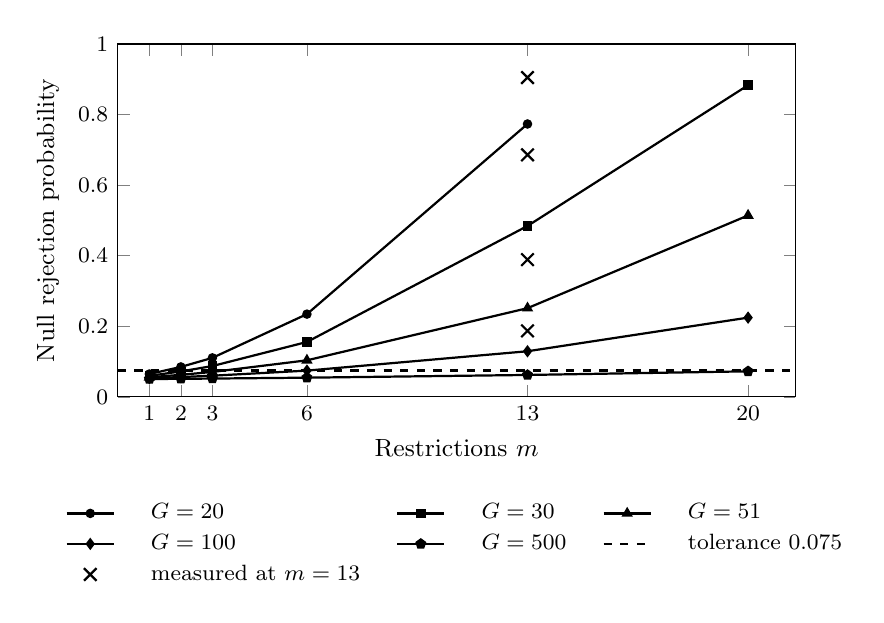
\begin{tikzpicture}
\begin{axis}[
  width=0.84\textwidth, height=0.50\textwidth,
  xlabel={Restrictions $m$},
  ylabel={Null rejection probability},
  xmin=0, xmax=21.5, ymin=0, ymax=1,
  xtick={1,2,3,6,13,20},
  ytick={0,0.2,0.4,0.6,0.8,1.0},
  legend cell align=left,
  legend columns=3,
  legend style={font=\footnotesize, draw=none, fill=none,
    at={(0.5,-0.27)}, anchor=north, column sep=1.1em},
  tick label style={font=\footnotesize},
  label style={font=\small},
]
\addplot[thick, mark=*, mark size=1.3] coordinates
  {(1,0.0648) (2,0.0849) (3,0.1106) (6,0.2345) (13,0.7734)};
\addlegendentry{$G = 20$}
\addplot[thick, mark=square*, mark size=1.3] coordinates
  {(1,0.0597) (2,0.0721) (3,0.0874) (6,0.1556) (13,0.4844) (20,0.8833)};
\addlegendentry{$G = 30$}
\addplot[thick, mark=triangle*, mark size=1.6] coordinates
  {(1,0.0556) (2,0.0625) (3,0.0706) (6,0.1036) (13,0.2514) (20,0.5142)};
\addlegendentry{$G = 51$}
\addplot[thick, mark=diamond*, mark size=1.6] coordinates
  {(1,0.0528) (2,0.0562) (3,0.0600) (6,0.0744) (13,0.1293) (20,0.2246)};
\addlegendentry{$G = 100$}
\addplot[thick, mark=pentagon*, mark size=1.6] coordinates
  {(1,0.0506) (2,0.0512) (3,0.0519) (6,0.0544) (13,0.0621) (20,0.0724)};
\addlegendentry{$G = 500$}
\addplot[dashed, thick, mark=none, domain=0:21.5, samples=2] {0.075};
\addlegendentry{tolerance $0.075$}
\addplot[only marks, mark=x, mark size=3.2, thick] coordinates
  {(13,0.905) (13,0.686) (13,0.389) (13,0.187)};
\addlegendentry{measured at $m = 13$}
\end{axis}
\end{tikzpicture}

\caption{Exact size of the nominal $5\%$ chi-square test against the number of
restrictions}
\label{fig:sizem}

\smallskip
\begin{minipage}{0.95\textwidth}
\footnotesize Notes: each curve gives the rejection probability of the nominal
level-$0.05$ chi-square test of the joint null $H_0: \gamma_P = 0$ in
(4.2), computed from (5.2) under Assumptions 2
and 3 at $\omega_2 = 1$, against the number of restrictions $m$, at
five cluster counts $G$. The dashed line marks a tolerance of $0.075$. The
crosses are the measured rejection rates at $m = 13$ and $C = 5$ from Table
2, at $G = 20$, $30$, $51$ and $100$ reading down, over $2{,}000$
replications each with a Monte Carlo standard error of at most $0.011$. They
lie above the corresponding curves because the simulated design gives
$G_{\mathrm{eff}}$ between $0.7142\,G$ and $0.7273\,G$ rather than the
equal cluster weights of
Assumption 3(ii). Sources:
\texttt{results/inference/anatomy\_expansion.csv},
\texttt{results/inference/size\_table.csv} and
\texttt{results/inference/anatomy\_effective\_clusters.csv}.
\end{minipage}
\end{figure}

\section{Staggered adoption}
\label{app:staggered}

Proposition 1 is stated for a single adoption cohort. The
construction behind it is a statement about one cohort's pre period, and with
several cohorts the comparisons that identify a later cohort before it adopts
can involve units that have already adopted and therefore already carry the
recording wedge. If that channel leaves a pre-period signature, a pre-period calibration can see the recording response after all and the blindness result is
weaker under staggering than Table 1 suggests.

Table \ref{tab:stag} settles the question by simulation. It repeats the
experiment of Table 1 with one change: three cohorts adopt at
periods $6$, $8$ and $10$ with $40$ percent of units never treated, in place of
one cohort adopting at period $8$ with half the units never treated. The
estimator, the reference implementation of the honest sets, the calibration of
the smoothness bound, the latent effect, the recording wedge and the target
horizon are all held fixed, so the two tables are comparable cell for cell.

\begin{table}[t]
\centering
\caption{Coverage of the latent effect under a recording response, staggered
adoption. Three cohorts adopting at periods $6$, $8$ and $10$, $40$ percent
never treated, latent effect $1.0$, recording wedge $0.6$ at the target horizon,
nominal $95\%$. The column $\max|\hat\beta_{\mathrm{pre}}|$ is the mean over
replications of the largest pre-treatment event-study coefficient in absolute
value. Everything else follows Table 1. Source:
\texttt{results/coverage/coverage\_staggered.json}, produced by
\texttt{scripts/oa\_staggered.py}.}
\label{tab:stag}
\begin{tabular}{rrrrccccc}
\toprule
& & & & \multicolumn{3}{c}{$\Delta^{\mathrm{RM}}(\bar M)$}
& \multicolumn{2}{c}{$\Delta^{\mathrm{SD}}(M)$} \\
\cmidrule(lr){5-7}\cmidrule(lr){8-9}
$N$ & reps & $\widehat M$ & $\max|\hat\beta_{\mathrm{pre}}|$
& $\bar M = 0.5$ & $\bar M = 1$ & $\bar M = 2$
& $M = \widehat M$ & institutional \\
\midrule
$400$ & $200$ & $0.5376$ & $0.1541$ & $0.300$ & $0.735$ & $0.955$ & $1.000$ & $1.000$ \\
$1{,}600$ & $200$ & $0.2729$ & $0.0727$ & $0.000$ & $0.150$ & $0.645$ & $1.000$ & $1.000$ \\
$6{,}400$ & $200$ & $0.1370$ & $0.0385$ & $0.000$ & $0.000$ & $0.085$ & $1.000$ & $1.000$ \\
$25{,}600$ & $100$ & $0.0653$ & $0.0187$ & $0.000$ & $0.000$ & $0.000$ & $0.880$ & $1.000$ \\
$102{,}400$ & $50$ & $0.0344$ & $0.0095$ & $0.000$ & $0.000$ & $0.000$ & $0.040$ & $1.000$ \\
\bottomrule
\end{tabular}
\end{table}

The collapse is the same and arrives sooner. Every relative magnitudes column
reaches zero coverage of the latent effect one sample size earlier than it does
in Table 1, the smoothness class calibrated from the pre-period fails at $N = 102{,}400$ rather than at $N = 409{,}600$, and the bound set from
the recording institution holds at $1.000$ throughout. The calibrated bound
$\widehat M$ is smaller at every sample size than its single cohort counterpart,
which is why the crossing happens earlier: a smaller bound admits a narrower
set, and the set has to contain a latent effect the recorded coefficients are
displaced away from.

The fourth column is what rules the contamination channel out. If the recording
response reached the pre-period through already-treated comparison units, the
largest pre-treatment coefficient would settle at a nonzero constant. It does
not. Multiplying it by $\sqrt{N}$ gives $3.081$, $2.908$, $3.082$, $2.992$ and
$3.034$ down the five rows, flat across a $256$ fold range of the panel size, so
the pre-period carries sampling noise and nothing else. At the largest panel the
recording wedge is $63$ times the largest pre-treatment coefficient it produces.

This is evidence rather than proof, and Proposition 1 remains stated
for one cohort. What the table removes is the possibility that staggering is
what rescues the pre period, which is the reading a reader of the scope
restriction might otherwise reach.


\begin{thebibliography}{99}

\bibitem[Armstrong and Koles\'ar(2018)]{armstrong2018optimal} Armstrong, T.~B., and Koles\'ar, M. (2018), ``Optimal Inference in a Class of Regression Models,'' \emph{Econometrica}, 86, 655--683.

\bibitem[Armstrong and Koles\'ar(2020)]{armstrong2020simple} Armstrong, T.~B., and Koles\'ar, M. (2020), ``Simple and Honest Confidence Intervals in Nonparametric Regression,'' \emph{Quantitative Economics}, 11, 1--39.

\bibitem[Arora and Chand(2026)]{arora2026trading} Arora, P., and Chand, A. (2026), ``Trading Scope for Credibility in Difference-in-differences,'', arXiv:2608.16867.

\bibitem[Baum et al.(2026)]{baum2026syphilis} Baum, A., Agha, L., Menzies, N., and Cohen, A. (2026), ``Prenatal Syphilis Screening Mandates and Maternal Syphilis Case Detection,'' \emph{JAMA Health Forum}, 7, e260123.

\bibitem[Bell and McCaffrey(2002)]{bell2002bias} Bell, R.~M., and McCaffrey, D.~F. (2002), ``Bias Reduction in Standard Errors for Linear Regression With Multi-stage Samples,'' \emph{Survey Methodology}, 28, 169--181.

\bibitem[Bester et al.(2011)]{bester2011cluster} Bester, C.~A., Conley, T.~G., and Hansen, C.~B. (2011), ``Inference With Dependent Data Using Cluster Covariance Estimators,'' \emph{Journal of Econometrics}, 165, 137--151.

\bibitem[Cai and Low(2004)]{cailow2004adaptation} Cai, T.~T., and Low, M.~G. (2004), ``An Adaptation Theory for Nonparametric Confidence Intervals,'' \emph{The Annals of Statistics}, 32, 1805--1840.

\bibitem[Calhoun(2011)]{calhoun2011testing} Calhoun, G. (2011), ``Hypothesis Testing in Linear Regression When $k/n$ is Large,'' \emph{Journal of Econometrics}, 165, 163--174.

\bibitem[Callaway and Li(2023)]{callaway2023pandemic} Callaway, B., and Li, T. (2023), ``Policy Evaluation During a Pandemic,'' \emph{Journal of Econometrics}, 236, 105454.

\bibitem[Cameron et al.(2008)]{cameron2008bootstrap} Cameron, A.~C., Gelbach, J.~B., and Miller, D.~L. (2008), ``Bootstrap-based Improvements for Inference With Clustered Errors,'' \emph{Review of Economics and Statistics}, 90, 414--427.

\bibitem[Campbell and Stanley(1963)]{campbell1963experimental} Campbell, D.~T., and Stanley, J.~C. (1963), \emph{Experimental and Quasi-Experimental Designs for Research}, Chicago: Rand McNally.

\bibitem[Canay et al.(2017)]{canay2017randomization} Canay, I.~A., Romano, J.~P., and Shaikh, A.~M. (2017), ``Randomization Tests Under an Approximate Symmetry Assumption,'' \emph{Econometrica}, 85, 1013--1030.

\bibitem[Carter et al.(2017)]{carter2017cluster} Carter, A.~V., Schnepel, K.~T., and Steigerwald, D.~G. (2017), ``Asymptotic Behavior of a $t$-test Robust to Cluster Heterogeneity,'' \emph{Review of Economics and Statistics}, 99, 698--709.

\bibitem[Denteh and K\'edagni(2022)]{denteh2022misclassdid} Denteh, A., and K\'edagni, D. (2022), ``Misclassification in Difference-in-differences Models,'', arXiv:2207.11890.

\bibitem[DiCiccio and Romano(2017)]{diciccio2017robust} DiCiccio, C.~J., and Romano, J.~P. (2017), ``Robust Permutation Tests for Correlation and Regression Coefficients,'' \emph{Journal of the American Statistical Association}, 112, 1211--1220.

\bibitem[Djogbenou et al.(2019)]{djogbenou2019asymptotic} Djogbenou, A.~A., MacKinnon, J.~G., and M.~{\O}. Nielsen (2019), ``Asymptotic Theory and Wild Bootstrap Inference With Clustered Errors,'' \emph{Journal of Econometrics}, 212, 393--412.

\bibitem[Fenaroli(2026)]{fenaroli2026joint} Fenaroli, F. (2026), ``A Joint Analysis of Sensitivity to Anticipation and Parallel Trends Violations,'', arXiv:2603.00868.

\bibitem[Freyaldenhoven et al.(2019)]{fhs2019pretrends} Freyaldenhoven, S., Hansen, C., and Shapiro, J.~M. (2019), ``Pre-event Trends in the Panel Event-study Design,'' \emph{American Economic Review}, 109, 3307--3338.

\bibitem[Freeman(2026)]{freeman2026local} Freeman, H. (2026), ``Local Asymptotic Power of Honest Confidence Intervals,'', arXiv:2607.10558.

\bibitem[Geruso and Layton(2020)]{geruso2020upcoding} Geruso, M., and Layton, T. (2020), ``Upcoding: Evidence From Medicare on Squishy Risk Adjustment,'' \emph{Journal of Political Economy}, 128, 984--1026.

\bibitem[Ghanem et al.(2026)]{ghanem2026when} Ghanem, D., Sant'Anna, P.~H.~C., and W\"uthrich, K. (2026), ``When Should Pre-trends Be Parallel? \emph{AEA Papers and Proceedings},''.

\bibitem[Goodman-Bacon and Marcus(2020)]{goodmanbacon2020covid} Goodman-Bacon, A., and Marcus, J. (2020), ``Using Difference-in-differences to Identify Causal Effects of COVID-19 Policies,'' \emph{Survey Research Methods}, 14, 153--158.

\bibitem[Gutknecht and Liu(2024)]{gutknecht2024cic} Gutknecht, D., and Liu, C. (2024), ``Changes-in-changes for Ordered Choice Models With Underreporting,'', arXiv:2401.00618.

\bibitem[Harasztosi and Lindner(2019)]{harasztosi2019minwage} Harasztosi, P., and Lindner, A. (2019), ``Who Pays for the Minimum Wage? \emph{American Economic Review} 109(8), 2693--2727,''.

\bibitem[Hausman et al.(1998)]{hausman1998misclassification} Hausman, J.~A., Abrevaya, J., and Scott-Morton, F.~M. (1998), ``Misclassification of the Dependent Variable in a Discrete-response Setting,'' \emph{Journal of Econometrics}, 87, 239--269.

\bibitem[Hotelling(1931)]{hotelling1931} Hotelling, H. (1931), ``The Generalization of Student's Ratio,'' \emph{Annals of Mathematical Statistics}, 2, 360--378.

\bibitem[Ibragimov and M\"uller(2010)]{ibragimov2010tstat} Ibragimov, R., and M\"uller, U.~K. (2010), ``$t$-statistic Based Correlation and Heterogeneity Robust Inference,'' \emph{Journal of Business \& Economic Statistics}, 28, 453--468.

\bibitem[Imbens and Koles\'ar(2016)]{imbens2016robust} Imbens, G.~W., and Koles\'ar, M. (2016), ``Robust Standard Errors in Small Samples: Some Practical Advice,'' \emph{Review of Economics and Statistics}, 98, 701--712.

\bibitem[Kahn-Lang and Lang(2020)]{kahnlang2020promise} Kahn-Lang, A., and Lang, K. (2020), ``The Promise and Pitfalls of Differences-in-differences: Reflections on 16 and Pregnant and Other Applications,'' \emph{Journal of Business \& Economic Statistics}, 38, 613--620.

\bibitem[Koles\'ar and Rothe(2018)]{kolesar2018discrete} Koles\'ar, M., and Rothe, C. (2018), ``Inference in Regression Discontinuity Designs With a Discrete Running Variable,'' \emph{American Economic Review}, 108, 2277--2304.

\bibitem[Kud\^o(1963)]{kudo1963} Kud\^o, A. (1963), ``A Multivariate Analogue of the One-sided Test,'' \emph{Biometrika}, 50(3--4), 403--418.

\bibitem[Lehmann and Romano(2005)]{lehmann2005testing} Lehmann, E.~L., and Romano, J.~P. (2005), \emph{Testing Statistical Hypotheses}, (3rd ed.). New York: Springer.

\bibitem[Low(1995)]{low1995bias} Low, M.~G. (1995), ``Bias-variance Tradeoffs in Functional Estimation Problems,'' \emph{The Annals of Statistics}, 23, 824--835.

\bibitem[Low(1997)]{low1997nonparametric} Low, M.~G. (1997), ``On Nonparametric Confidence Intervals,'' \emph{The Annals of Statistics}, 25, 2547--2554.

\bibitem[MacKinnon and Webb(2017)]{mackinnon2017wild} MacKinnon, J.~G., and Webb, M.~D. (2017), ``Wild Bootstrap Inference for Wildly Different Cluster Sizes,'' \emph{Journal of Applied Econometrics}, 32, 233--254.

\bibitem[MacKinnon et al.(2023)]{mackinnon2023guide} MacKinnon, J.~G., M.~{\O}. Nielsen, and Webb, M.~D. (2023), ``Cluster-robust Inference: A Guide to Empirical Practice,'' \emph{Journal of Econometrics}, 232, 272--299.

\bibitem[Malani and Reif(2015)]{malani2015interpreting} Malani, A., and Reif, J. (2015), ``Interpreting Pre-trends as Anticipation: Impact on Estimated Treatment Effects From Tort Reform,'' \emph{Journal of Public Economics}, 124, 1--17.

\bibitem[Mikhaeil and Harshaw(2025)]{mikhaeil2025valid} Mikhaeil, J.~M., and Harshaw, C. (2025), ``Valid Inference When Testing Violations of Parallel Trends for Difference-in-differences,'', arXiv:2510.26470.

\bibitem[Pan and Wall(2002)]{panwall2002} Pan, W., and Wall, M.~M. (2002), ``Small-sample Adjustments in Using the Sandwich Variance Estimator in Generalized Estimating Equations,'' \emph{Statistics in Medicine}, 21, 1429--1441.

\bibitem[Pustejovsky and Tipton(2018)]{pustejovsky2018small} Pustejovsky, J.~E., and Tipton, E. (2018), ``Small-sample Methods for Cluster-robust Variance Estimation and Hypothesis Testing in Fixed Effects Models,'' \emph{Journal of Business \& Economic Statistics}, 36, 672--683.

\bibitem[Rambachan and Roth(2023)]{rambachan2023credible} Rambachan, A., and Roth, J. (2023), ``A More Credible Approach to Parallel Trends,'' \emph{Review of Economic Studies}, 90, 2555--2591.

\bibitem[Richardson et al.(2025)]{richardson2025ipv} Richardson, R., Raj, A., Downs, J., Bergenfeld, N., Wiltshire, R., Dimitrova, A., and Benmarhnia, T. (2025), ``Impact of Domestic Violence Legislation on Reported Intimate Partner Violence: A Difference-in-differences Analysis Across 16 Countries,'' \emph{SSM--Population Health}, 43, 101837.

\bibitem[Roth(2022)]{roth2022pretest} Roth, J. (2022), ``Pretest With Caution: Event-study Estimates After Testing for Parallel Trends,'' \emph{American Economic Review: Insights}, 4, 305--322.

\bibitem[Roth et al.(2023)]{roth2023trending} Roth, J., Sant'Anna, P.~H.~C., Bilinski, A., and Poe, J. (2023), ``What's Trending in Difference-in-differences? a Synthesis of the Recent Econometrics Literature,'' \emph{Journal of Econometrics}, 235, 2218--2244.

\bibitem[Shapiro(1988)]{shapiro1988} Shapiro, A. (1988), ``Towards a Unified Theory of Inequality Constrained Testing in Multivariate Analysis,'' \emph{International Statistical Review}, 56, 49--62.

\bibitem[Tipton and Pustejovsky(2015)]{tipton2015small} Tipton, E., and Pustejovsky, J.~E. (2015), ``Small-sample Adjustments for Tests of Moderators and Model Fit Using Robust Variance Estimation in Meta-regression,'' \emph{Journal of Educational and Behavioral Statistics}, 40, 604--634.

\bibitem[Weisburd et al.(2024)]{weisburd2024crs} Weisburd, D., Wilson, D.~B., Gill, C., Kuen, K., and Zastrow, T. (2024), ``Are We Underestimating the Crime Prevention Outcomes of Community Policing? the Importance of Crime Reporting Sensitivity Bias,'' \emph{Journal of Law and Empirical Analysis}, 1, 1--17.

\bibitem[Young(2019)]{young2019fisher} Young, A. (2019), ``Channeling Fisher: Randomization Tests and the Statistical Insignificance of Seemingly Significant Experimental Results,'' \emph{Quarterly Journal of Economics}, 134, 557--598.

\end{thebibliography}

\end{document}

